\documentclass{report}
\usepackage[utf8]{inputenc}
\usepackage{float}
\usepackage[T1]{fontenc}
\usepackage[normalem]{ulem}
\usepackage[nottoc,notlof,notlot]{tocbibind}
\usepackage{algorithm}
\usepackage{algorithmic}
\usepackage{graphicx}
\title{Compared analysis of taxonomic trees}
\author{C. REDA \\ \\ supervised by M. NIKOLSKI and M. RAFFINOT\\CBIB, Bordeaux}
\date{August, 21 2016}
\begin{document}

\maketitle

\chapter*{Abstract}
\nocite{*}
Taxonomic trees -also called phylogenetic trees- are trees that represent the classification of species into groups according to their evolutionnary past. In metagenomics, that is the study of genetic material from samples taken from a natural environment (opposite to labs), taxonomic trees allow to identify the species matching the samples, and thus to determine the composition of the microbial population endemic to the environment.\\

Interest in metagenomics has recently plummeted in bioinformatics, as a consequence of the decreasing price of DNA sequencing, and also for studying environmental samples has unveiled the existence of many bacterias which could not be cultivated in labs. Metagenomics has got many applications to biology and medicine. The subject of this internship is to enhance the extraction of data from the genetic material for medical purposes.\\

\newpage
 
\tableofcontents
 
\newpage

\listoffigures

\newpage

\listoftables

\newpage
 
\pagenumbering{arabic}

\chapter{Scientific context}

Firstly we will explain what metagenomics is, how taxonomic trees intervene in this scientific field, and what are the most burning issues today in metagenomics. Then we will introduce the test database.

\section{Definition and goals of metagenomics}
Metagenomics is the study of the genetic material of samples directly taken from a natural environment. It can be parts of DNA, proteins or RNA.\\

We only focus here on bacteria's DNAs. Indeed bacteria used to be cultivated in laboratories before having their DNA sequenced and annoted. However a great number of bacteria cannot be raised in an artificial environment, such as some bacteria in animal guts or living in fragile marine ecosystems. Thus metagenomics helps to study more and new species of bacteria. Along with the decreasing price of DNA sequencing, this explains the development and the growing interest in metagenomics today.\\

The whole pipeline to turn raw genetic material into reliable data comprises these following steps:
\begin{itemize}
\item After removing samples of genetic data from the environment, one extracts the DNA from the sample by a chemical reaction
\item Then one sequences the resulting DNA, that is to say one searches the structure of the DNA, i.e. the order of (set of) the base pairs constructed with cytosine ($\{C\}$), adenine ($\{A\}$), guanine ($\{G\}$), and thymine ($\{T\}$), that encodes the necessary information for the living of organisms. Note that there exists other bases such as $N = \{A,C,T,G\}$ or $X$, and this fact increases greatly the complexity of sequencing. There are two ways of sequencing: the first method is the slowest, but give good quality lecture of the DNA, and is mainly used to generate reference genomes. The second one (\textsc{NGS}, that stands for \textsc{Next-Generation Sequencing} \cite{WikiNGS}) is faster, and can give errors. This last method targets only parts of the DNA, of length 32 to 1,000 base pairs, unlike the first one that would sequence the whole DNA.
\end{itemize}

For bacteria, only some parts of the DNA change from a bacterium to another (these parts are called \emph{hyper variable regions} or \emph{HVR}), while some remain the same for all bacteria. The sequencing therefore focuses on the \emph{HVR} to seek the nature of the bacteria to which the read belongs. It is particularly hard to correctly determine the bounds of these \emph{HVR}, and it is one of the causes of error in sequencing.\\

Once the sequencing by \textsc{NGS} is done, one obtains \emph{reads} -annoted bits of DNA sequences of length 32 to 1,000 base pairs:\\

e.g. this (partial) read is associated to the \emph{16S} gene of species \emph{Hydrothermal vent clone VC2.1 Arc13}; the \emph{16S} gene is strongly related to the species of the bacterium:\\
\begin{center}
AGGCCACTGCTATCGGGCTCCGACTAAGCCATGCGAGTCTAG\\
GGGCTCCTTCGGGAGCACCGGCGGACGGCTCAGTAACACGTGGACAA\\
CCTACCCTCGGGTGGGGGATAACCTCGGGAAACTGAGGCTAATACCC...\\
\end{center}

These reads are then usually matched with the reference sequences found in databases such as \textsc{NCBI}, \textsc{GreenGenes} or \textsc{RDP}: for one read, one looks for the best alignment with one of the reference sequences, somehow the alignment that preserves most the order of the bases (see figure $1.1$). After this step, in the case of human bacteria (unfortunately it is not a general rule), to one read corresponds one or more sequences, that is, one or more species.\\

\begin{figure}[H]
\centering
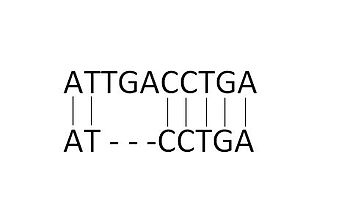
\includegraphics[scale=0.5]{illustrations/Sequence_gaps.JPG}
\caption{An example of alignment of DNA sequence, from \emph{Gap penalty} article in \textsc{Wikipedia}}
\end{figure}

The main objective of metagenomics is to then extract the maximum of relevant information from the obtained reads and from the matching to the reference sequences.

\section{Assignment/identification of reads to a certain species of bacteria}

There exists no unique common phylogeny. A handful of phylogenetic trees are used in bioinformatics, coming from different databases such as, for instance, \textsc{NCBI}, \textsc{GreenGenes} or \textsc{RDP}.\\

A taxonomic tree (see figure $1.2$) is of bounded height, which value can vary according to the database associated. In \textsc{GreenGenes}'s phylogenetic tree, that is the one used for the tests, there are eight ranks, that is, eight levels/generations in the tree in growing precision (see figure $3$):
\begin{itemize}
\item 'D' (\textsc{Domain}) or 'R' (\textsc{Reign}): this rank is basically divided into three nodes: '\emph{Bacteria}', '\emph{Archae}' and '\emph{Eucarya}'.
\item 'P' (\textsc{Phylum}): '\emph{Animalia}', '\emph{Plantae}', '\emph{Fungi}', ...
\item 'C' (\textsc{Class}): '\emph{Mammalia}', ...
\item 'O' (\textsc{Order}): '\emph{Carnivora}', ...
\item 'F' (\textsc{Family}): '\emph{Carnidae}', ...
\item 'G' (\textsc{Genus}): '\emph{Vulpes}', ...
\item 'S' (\textsc{Species}): '\emph{Vulpes}', ... (corresponds to a single species)
\end{itemize} 


\begin{figure}[H]
\begin{center}
\subfigure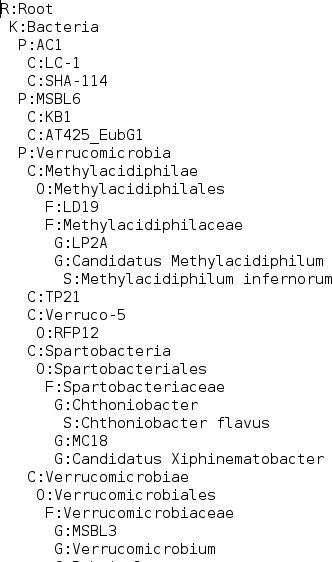
\includegraphics[scale=0.35]{illustrations/arbretaxo.png}
\subfigure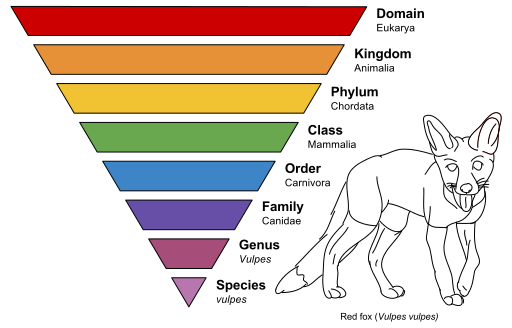
\includegraphics[scale=0.35]{illustrations/Taxonomic_Rank.png}
\caption{A partial taxonomic tree from \textsc{GreenGenes} and the taxonomy of the fox, from \emph{Taxonomic Rank} article in \textsc{Wikipedia}}
\end{center}
\end{figure}

It is worth noticing that the nearest nodes to the root have got the lowest degree, and that a taxonomic tree has a great proportion of leaves (S-ranked nodes) compared to the number of nodes. \textsc{GreenGenes}'s taxonomic trees for the domains '\emph{Bacteria}' and '\emph{Archae}' approximately owns $9,065$ nodes, and among them $5,565$ leaves.\\

Most of the time, since many species could have matched one read, reads are assigned to a very one node of the taxonomic tree. Generally speaking, a read is assigned to the \emph{Least Common Ancestor} (\textsc{LCA}) \cite{Tarjan} of the set of matched sequences/species/S-ranked nodes. The \textsc{LCA} of a set of leaves S is the last common node in the paths from the root to each leaf of S.

\begin{figure}[H]
\centering
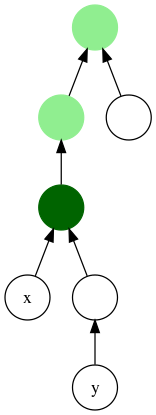
\includegraphics[scale=0.35]{illustrations/Lowest_common_ancestor.png}
\caption{The dark green node is the LCA of \emph{x} and \emph{y}, from \emph{Lowest Common Ancestor} article in \textsc{Wikipedia}}
\end{figure}

One can seldomly associate one read to a single species, because of errors in the sequencing. The deeper in the tree the read is assigned, the best it is. Nevertheless, some algorithms to improve the accuracy of assignment of reads have been designed \cite{Tango1} \cite{Tango3}. Please note eventually that a node can match several reads from a same sample, and thus several reads can be assigned to this node in a single sample.

\section{Topics in metagenomics}

There are already algorithms that enhance the assignment of a read to a node of the taxonomic tree \cite{Tango1}, and measures on phylogenies that quantify the relevancy of the tree according to a certain distance matrix between reads, or according to a certain other taxonomic tree \cite{RobinsonFoulds} \cite{Alignment}. But one lacks of efficient tools \cite{Enaud} when it comes to compare several trees/forests by quantifiying their similarities and also their differences, and above all to draw biological conclusions on the presence or the absence of certain nodes, provided some metadata.\\

For instance, given a group of patients afflicted with cystic fibrosis, one can extract samples from their guts and may want to evaluate the influence of the age or the treatment over the population of \emph{E. Coli} bacteria in their patient's guts. Statistics methods, using e.g. \textsc{Wilcoxon} \cite{Wilcoxon} \cite{Whitney} or \textsc{Mc Nemar}'s \cite{McNemar} tests, are nowadays used to answer these questions, but their interpretation needs a manual overlap of the analysed data. To guide the diagnosis or the evaluation of the efficiency of a treatment, practitionners are in need of a semi-automatic processing of the data.

\section{The test database}

The test database used to design the algorithms is a study which took place at the Children's Hospital of Bordeaux, from November, 2015 to May, 2016 \cite{Enaud}. All patients were afflicted with cystic fibrosis, and some of them needed a heavy antibacterial treatment by intraveinous injection (denoted ATB-IV) to cure their chronic bacterial infections. The aim of the study was to underline the influence of antibacterials on the microbial population of the patient's gut.\\

Patients were divided into witnesses (\textsc{W}) and treated patients (\textsc{T}). These ones in the \textsc{W} group saw the paediatrician twice, on Day $0$ and Day $90$. The ones in the \textsc{T} group saw him thrice, on Day $0$, Day $45$ and Day $90$, and were treated from Day $0$ to Day $45$. There are in total $47$ samples, with $21$ patients.\\

Each time patients saw the doctor, they gave them samples of their stools and a filled survey over their quality of life. Samples were then sequenced. Later on, results were filtered and normalized this way:

\begin{itemize}
\item Variables that will not likely be useful (e.g. a node with a number of assignments too small) are identified and removed: for instance, if the number of assignments falls below the first quartile, the variable associated is discarded
\item Assignment numbers have been normalized relatively to the total number of reads assigned in the taxonomic tree
\item Then these numbers have been mean-centered and reduced
\end{itemize}

\newpage

\chapter{Subject of the internship}

The research aimed at answering two quite similar problems, that mainly target at \emph{clustering} patients, that separates them into groups which maximize the resemblance between two patients of a same group or \emph{cluster}, and minimize it for a pair of patients from different \emph{clusters}. For all these problems, a common numerotation of the samples, the nodes in the taxonomic tree, and the metadata had been chosen. Furthermore, we use for input a reference taxonomic tree denoted \textsc{T} (from GreenGenes's in our test database), and a \emph{data/information matrix} denoted \textsc{infoM}, such as \textsc{infoM}[$i$][$j$] is the value of metadatum $j$ in sample $i$ (being $0$ or $1$ for boolean values). 

\section{Problem of most different pairs (MDP)}
\textsc{MDP} is:\\

\textsc{Supplementary input:} 
                \begin{itemize}
                \item A matrix \textsc{occM} (called \emph{occurrence matrix}) such as \textsc{occM}[$i$][$j$] is the number of assignments to node $j$ in sample $i$
                \item A set of groups of samples \textsc{S}
                \end{itemize}

\bigskip

\textsc{Output:} \begin{itemize}
                 \item The list of the pairs in \textsc{S} that are the most different
                 \end{itemize}

\begin{figure}[H]
\centering
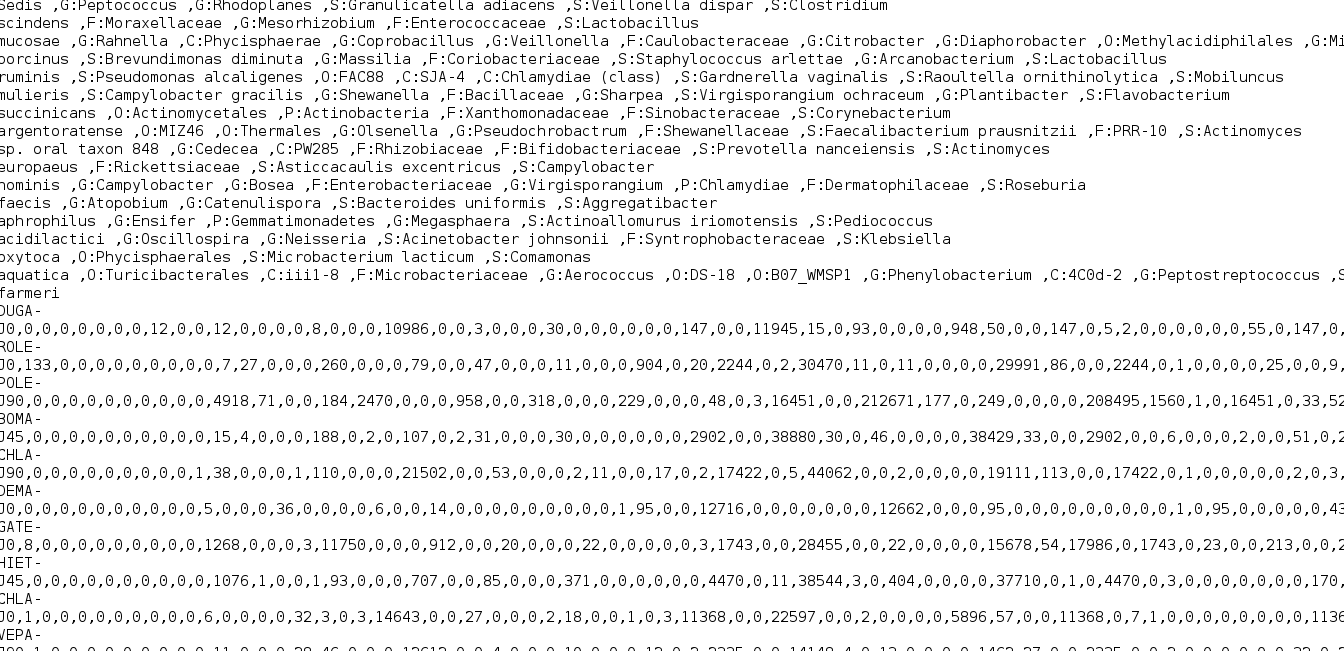
\includegraphics[scale=0.3]{illustrations/occmatrix.png} 
\caption{A screenshot of the occurrence matrix from the test database}
\end{figure}

\begin{figure}[H]
\centering
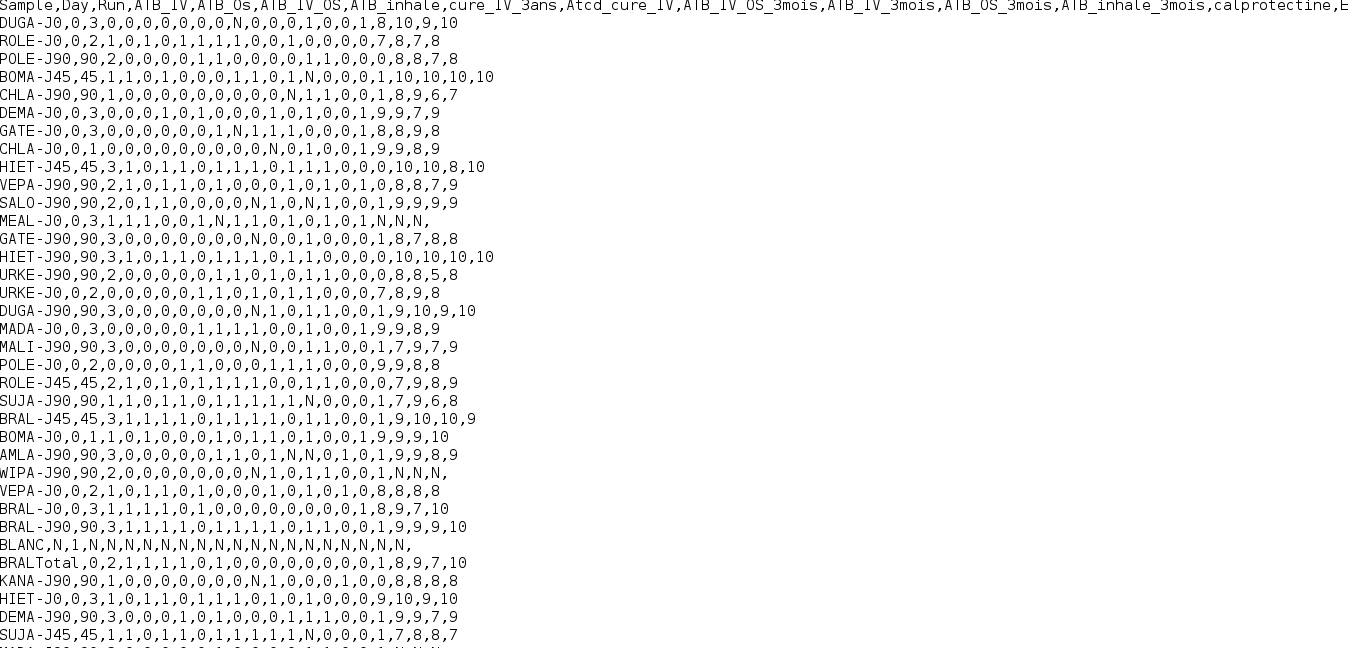
\includegraphics[scale=0.3]{illustrations/infomatrix.png}
\caption{A screenshot of the info matrix from the test database}
\end{figure}

\section{Problems of clustering (CL)}

The following two problems deal with the clustering of the groups of samples by their respective microbial populations, and the comparison of such a clustering with the values of metadata for these groups, in order to find a potential correspondance between bacteria and metadata. 

\subsection{Problem of compatibility (CL.C)}
\textsc{CL.C} is:\\

\textsc{Supplementary input:} \begin{itemize}
                \item The set of lists of nodes \textsc{nodesS} (called \emph{matchingNodes}) such as \textsc{nodesS}[$i$] is the list of nodes matched in at least one of the reads in sample $i$
                \item A subset \textsc{N} of the set of nodes in the taxonomic tree
                \item A set of metadata \textsc{M}
                \end{itemize}

\bigskip

\textsc{Output:} \begin{itemize}
                 \item Decide if the clustering of samples according to the microbial population restricted to \textsc{N} is compatible with the clustering of samples according to their values of metadata in \textsc{M}.
                 \end{itemize}

\subsection{Problem of best clustering (CL.BCL)}
\textsc{CL.BCL} is:\\

\textsc{Supplementary input:} 
                \begin{itemize}
                \item The set of lists of nodes \textsc{nodesS} (called \emph{matchingNodes}) such as \textsc{nodesS}[$i$] is the list of nodes matched in at least one of the reads in sample $i$
                \item A set of metadata \textsc{M}
                \end{itemize}

\bigskip

\textsc{Output:} \begin{itemize}
                 \item Find the best subset \textsc{N} of the set of nodes in \textsc{T} for a compatible classification of samples according to values of metadata in \textsc{M}.
                 \end{itemize}

\newpage

\chapter*{Methods}

Three different approaches have been designed, each of them answering one of these problems. In chronological order:
\begin{itemize}
\item Firstly, a method using statistical approach, with customized measures on microbial populations, determines a distance between the samples to solve problem $1$. However, this method needs robust measures to be relevant, and the biological phenomena are not so easy to describe with only a few characteristics.
\item A second approach uses the \emph{supervised learning} paradigm, and tries to identify nodes (of the taxonomic tree)/bacteria that discriminate the samples the way the values of metadata do, that is, finds the nodes which seem to have a relationship with the considered metadata. Nevertheless, strong \emph{a priori} hypotheses on microbial populations have to be made, which could bias the results.
\item Eventually, another method uses \emph{non-supervised learning}. It clusters the samples with two distances only depending on node populations, and compares the resulting clusters with the groups of metadata values.
\end{itemize}
The first and third methods use a special implementation of taxonomic trees (see annex \textsc{C}).

\chapter{Statistical-like approach}

\section{Definitions}

There are a few useful definitions to know:
\begin{enumerate}
\item \textsc{A tree induced by a group of samples G} is the tree (or the forest) containing only nodes that have been assigned at least once in one of the samples in \textsc{G}.

\begin{figure}[H]
\centering
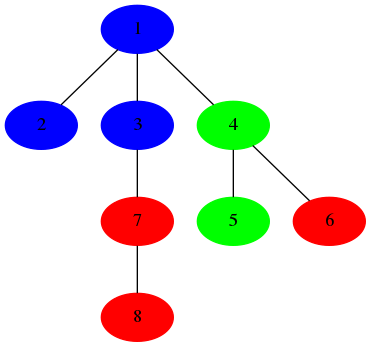
\includegraphics[scale=0.5]{illustrations/inducedtree.png}
\caption{Subtrees induced by three groups of samples (each corresponding to a single colour). Incuced subtrees can of course overlap.}
\end{figure}

\item \textsc{A pattern in the tree A} is a connex subgraph of \textsc{A}. For instance, the blue tree from the example above.
\end{enumerate}

\newpage

\section{Description of the method}

This approach tries to answer the first problem, and computes a certain number of scores for a group of samples, independantly of the values of metadata. Each score corresponds to a partial definition of identity between two groups of samples. The union of those scores aims at quantifying the most accurately the difference between two sets of samples.

\subsection{Total Ratio}

\begin{itemize}
\item \textsc{Total Ratio:} provided two groups $G_{1}$ and $G_{2}$ of samples, if $n$ is the number of assignments to common nodes in both groups (i.e. the sum of assignments in common nodes in each group), and $n_{1}$ et $n_{2}$ respectively the number of assignments in these two groups in non-common nodes, then Total Ratio is $TR(1,2) = \frac{n}{n_{1} + n_{2} + n}$. If $n_{1} = n_{2} = n = 0$, it mean no read from the samples of $G_{1}$ and $G_{2}$ has matched a node in \textsc{T}. We choose to have in this case $TR = +\infty$.

\begin{figure}[H]
\centering
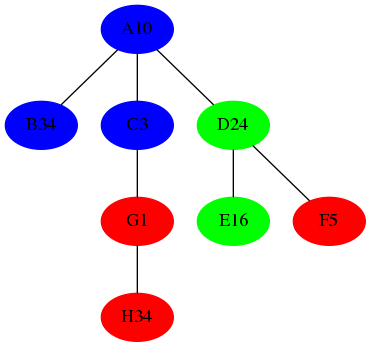
\includegraphics[scale=0.5]{illustrations/totalratio.png}
\caption{Example for \textsc{Total Ratio}: blue nodes are common to green and red trees. Green and red nodes correspond to two distinct groups of samples. Here, $TR$ = $\frac{10 + 3 + 34}{(1 + 34 + 5) + (10 + 3 + 34) + (24 + 16)} \simeq 0.37$}
\end{figure}

\bigskip

  \textsc{Biological interpretation:} Total Ratio Distance focuses on the node population in samples. If $n_{1} + n_{2} = 0$, it means that $G_{1}$ and $G_{2}$ have got the same set of nodes and thus $TR = 1$. If $TR = 0$, it means $G_{1}$ and $G_{2}$ have no node in common.
\end{itemize}

\subsection{Pattern Ratio}

\begin{itemize} 
\item \textsc{Pattern Ratio:} if $n$ is the number of assignments in common patterns of length > 1 in the trees induced by the groups $G_{1}$ and $G_{2}$ of samples selected, and $N$ the number of assignments in specific patterns, then Pattern Ratio is the quantity: $PR(1,2) = \frac{n}{M}$. If $M = 0$, it means the two trees induced by $G_{1}$ and $G_{2}$ are the same, so having $PR = +\infty$ is consistent.

\begin{figure}[H]
\centering
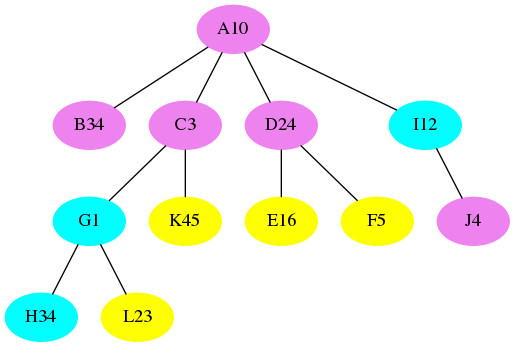
\includegraphics[scale=0.5]{illustrations/patternratio.png}
\caption{Example for \textsc{Pattern Ratio}: violet nodes are common to cyan and yellow trees. Cyan and yellow nodes correspond to two distinct groups of samples. Here, $PR$ = $\frac{10 + 34 + 3 + 24}{(1 + 34 + 12) + (23 + 45 + 16 + 5)} \simeq 0.52$}
\end{figure}

\bigskip

  \textsc{Biological interpretation:} Pattern Ratio rather focuses on the phylogenetic proximity between the nodes of the two groups. When computed for the whole set of samples, it corresponds to the 'functional kernel' of the gut, that is, a group of bacteria that is usually common to every human and that allow the different chemical reactions in the gut. 

\end{itemize}

\subsection{Microbial Diversity}

\begin{itemize}
\item \textsc{Microbial Diversity:} provided a group of samples $G$, if $n_{nodes}$ is the number of nodes in the tree induced by $G$, and $n_{tree}$ the number of nodes in the whole taxonomic tree, then Microbial Diversity is: $MD(G) = \frac{n_{nodes}}{n_{tree}}$. It is the definition of diversity used in \cite{Enaud}, that must be distinguished from \textsc{Phylogenetic Diversity} \cite{PhyloD} and \textsc{Mean Diversity} \cite{MeanD} coefficients.

\begin{figure}[H]
\centering
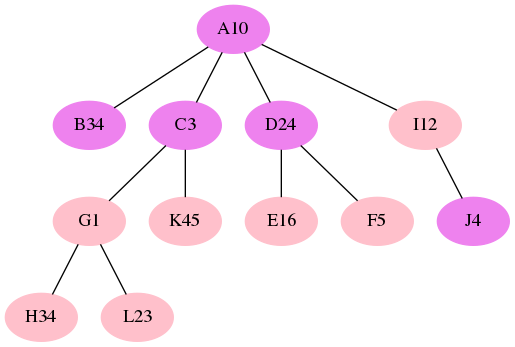
\includegraphics[scale=0.5]{illustrations/diversity.png}
\caption{Example for \textsc{Microbial Diversity}: Here, \textsc{Microbial Diversity} coefficient for violet tree is: $MD$ = $\frac{5}{12} \simeq 0.42$}
\end{figure}

\bigskip

\textsc{Biological interpretation:} The diversity of bacteria for instance in guts is of paramount importance, because the equilibrium of the ecosystem is compulsory to ensure the good development of the gut. Therefore two samples having the same sort of bacteria in different proportions must be considered different. This coefficient may be quite superfluous with the previous scores, but it seems justified by biology.

\end{itemize}

\subsection{Computation of the similarity coefficient}

The final similarity coefficient $s$ between two groups of samples $G_{1}$ and $G_{2}$ (distance $d$ can be obtained from s with the formula: $d = \frac{1}{s}$, $d = +\infty$ if $s = 0$) to compare the groups of patients is a mix of these scores. An equal importance here is accorded to each score in the following formula:\\

\begin{center}
if $MD(G_{1}) - MD(G_{2}) = 0$:\\
$s(G_{1},G_{2}) = TR(1,2) + PR(1,2)$\\

else:\\
$s(G_{1},G_{2}) = TR(1,2) + PR(1,2) - | MD(G_{1}) - MD(G_{2}) |$\\
\end{center}

Then this similarity coefficient is normalized:\\
\begin{center}
$\overline{s}(G_{1},G_{2}) = \frac{s(G_{1},G_{2}) - E(s)}{\sigma(s)}$\\
\end{center}

Then the program asks for a metadatum to cluster the set of samples in groups $(G_{i})_{i}$, each group corresponding to one single known value of the metadatum. After computing $\overline{s}$ for every pair of $(G_{i})_{i}$, it returns the list of pairs of groups $(G_{i},G_{j})_{i \neq j}$ such as $\overline{s}(G_{i},G_{j}) \le FQ$, where $FQ$ is the value of the first quartile. 

\section{Implementation}

The implementation of TaxoTree in \textsc{Python 2.9.7} offers a few other features:

\begin{enumerate}
\item After selection of a group of bacteria and of a group of samples/metadata, gives an array with the percentage of assignments to this family of bacteria depending on the samples/metadata
\item Computes the Pearson correlation coefficient $r$ between a number of assignments to a group of bacteria and a group of metadatas, or between the numbers of assignments to two groups of bacteria \\

\textsc{Pearson sample product-moment correlation coefficient:} \cite{Pearson} for vectors $x$ and $y$ of values of size $n$, if $\overline{x}$ is the mean of the $(x_{i})_{i}$, and $\overline{y}$ the mean of the $(y_{i})_{i}$, then $r = \frac{\sum{_{i = 1}^{n}}{(x_{i} - \overline{x}) \times (y_{i} - \overline{y})}}{\sqrt{\sum{_{i = 1}^{n}}{(x_{i} - \overline{x})^{2}}} \times \sqrt{\sum{_{i = 1}^{n}}{(y_{i} - \overline{y})^{2}}}}$. $r$ is comprised between $1$ and $-1$:
\begin{itemize} 
\item $r = 1$ meaning there is a perfect uphill linear relationship between $x$ and $y$
\item $r = -1$ meaning there is a perfect downhill linear relationship between $x$ and $y$
\item $r = 0$ meaning there is no linear relationship at all
\end{itemize}

\item Draws graphs and pie charts
\item Computes a distance coefficient $sim(k,l)$ between two patients $P_{k}$ and $P_{l}$: after selecting a subset $M' = \{ m_{i_{1}}, m_{i_{2}}, ... m_{i_{m}}\}$ of the set of metadata, if $n_{j,k}$ known value in $P_{k}$ for $m_{i_{j}}$, then $dist(k,l) = \sum{_{j = 1}^{m}}{|n_{j,k} - n_{j,l}|}$. The corresponding similarity coefficient is $sim(k,l) = \frac{1}{dist(k,l)}$, $sim(k,l) = +\infty$ iff $dist(k,l) = 0$.
\end{enumerate}

Code is available at: \emph{https://github.com/cbib/taxotree}.\\

The overall worst case time complexity of the computation of distance matrix is O($n_{taxo-nodes}^{2} \times n_{samples}^{3}$) (see annex for more details). On our computer (see annex for physical characteristics), it took 10 minutes to compute it.

\section{Results}

\subsection{Tests}

The results have been compared to those obtained by statistical methods on the test database (5):

\begin{itemize}
\item \textsc{Comparison of microbial populations at Day 0:} 
       \textsc{Output of the statistical analyses (chapter 5.2.2):} Microbial populations between groups of samples without antibacterials (samples selected with parameters $Day = 0$, $ATB-IV = 0$) and with antibacterials (samples selected with parameters $Day = 0$, $ATB-IV = 1$) are said to be very alike according to the statistical results of the study. \emph{Clostridium bolteae} and \emph{Pediococcus acidilactici} were overrepresented in $ATB-IV = 1$ groups.\\

According to the table and pie charts, the results seem to confirm the output of TaxoTree.

     \begin{table}
       \caption{Results from \textsc{TaxoTree} for the comparison at Day 0, (*) with Day = 0, (**) with (Clostridium bolteae,S),(Pediococcus acidilactici,S), where S is one of the taxonomic ranks}
       \begin{tabular}{|l|c|r|}
         \hline
         \textsc{Score} & \textsc{Result} & \textsc{Parameters}\\
         \hline
         Normalized Total Ratio & 0.92837592759 & ATB-IV=0,1 (*)\\
         \hline
         Pattern Ratio & 9.46867603736 & ATB-IV=0,1 (*)\\
         \hline
         Percentage Assignments & 59.954342\% & ATB-IV=1, option "bacteria" (**)\\
         \hline
         Percentage Assignments & 5.877773\% & ATB-IV=0, option "bacteria" (**)\\
         \hline
         Microbial Diversity & 0.0227222589896 & ATB-IV=0 (*) \\
         \hline
         Microbial Diversity & 0.0196337966027 & ATB-IV=1 (*) \\
         \hline
       \end{tabular}
     \end{table}
       
           \begin{figure}[H]
             \centering
             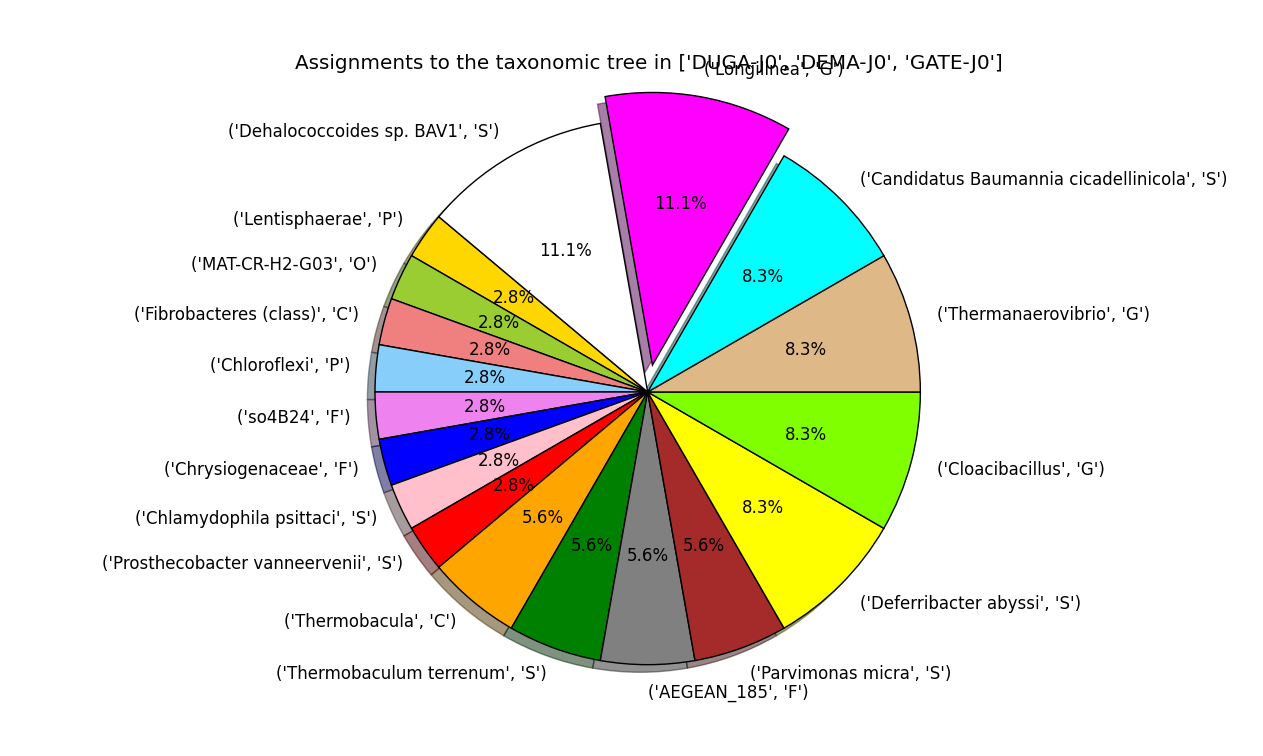
\includegraphics[scale=0.4]{illustrations/diversityDay0ATB0.png}
             \caption{Microbial Diversity Day=0, ATB-IV=0}
           \end{figure}

           \begin{figure}[H]
             \centering
             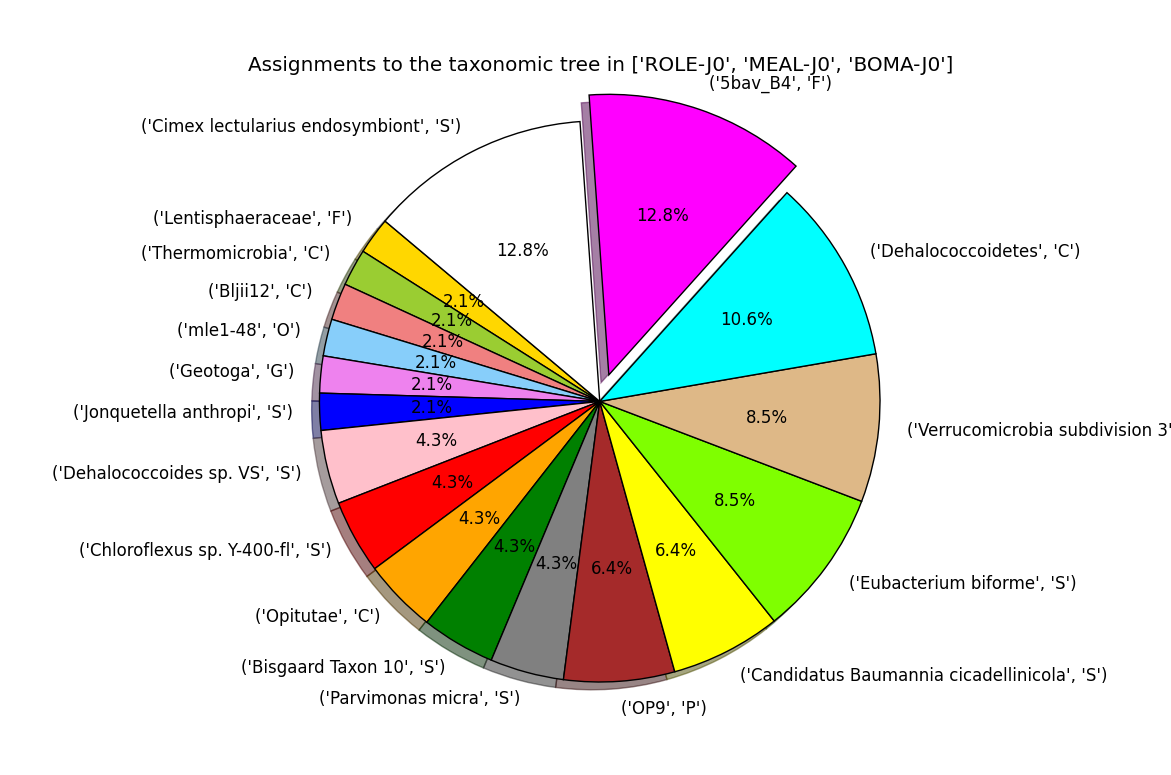
\includegraphics[scale=0.4]{illustrations/diversityDay0ATB1.png}
             \caption{Microbial Diversity Day=0, ATB-IV=1}
           \end{figure}
         \end{itemize}

\item \textsc{Evolution of microbial populations:}
       \textsc{Output of the statistical analyses (chapter 5.2.3):} Microbial populations are said to change between Day $0$, Day $45$ and Day $90$ for all patients, with/without $ATB-IV$. Nevertheless microbial diversity seemed not to be sensibly different between Day $0$, Day $45$ and Day $90$ in patients being treated with antibacterials.\\

The result of Total Ratio does not match the statistical results. However, Pattern Ratio does show the variations of the microbial populations between Day $0$, Day $45$ and Day $90$. Indeed, when Pattern Ratio is largely superior to $1$, it means the samples have similar node population and have got some similar clusters of nodes. It could mean patients' guts recover their initial $Day-0$ microbial population at Day $90$, that explains the high coefficient of similarity between Day $0$ and Day $90$ samples, while the $Day-45$ samples have got a different node population than initially due to the treatment and a unknown cause for untreated patients (the paper underlines this problem for $ATB-IV = 0$ patients). Microbial diversity seems not to really change between Day $0$, Day $45$ and Day $90$ for $ATB-IV = 1$ patients.

     \begin{table}
       \caption{Results from \textsc{TaxoTree} for the comparison at Day 0, Day 45, Day 90}
       \begin{tabular}{|l|c|r|}
         \hline
         \textsc{Score} & \textsc{Result} & \textsc{Parameters}\\
         \hline
         Normalized Total Ratio & 0.969346342836 & Day=0,45\\
         \hline
         Normalized Total Ratio & 0.929612804449 & Day=45,90\\
         \hline
         Normalized Total Ratio & 0.94998844733 & Day=0,90\\
         \hline
         Pattern Ratio & 3.75530416309 & Day=0,45 \\
         \hline
         Pattern Ratio & 13.0716519314 & Day=0,90 \\
         \hline
         Pattern Ratio & 1.9536860416 & Day=45,90 \\
         \hline
         Microbial Diversity & 0.0196337966027 & Day=0,ATB-IV=1 \\
         \hline
         Microbial Diversity & 0.0195234943746 & Day=45,ATB-IV=1 \\
         \hline
         Microbial Diversity & 0.0163247297595 & Day=90, ATB-IV=1\\
         \hline
       \end{tabular}
     \end{table}

           \begin{figure}[H]
             \centering
             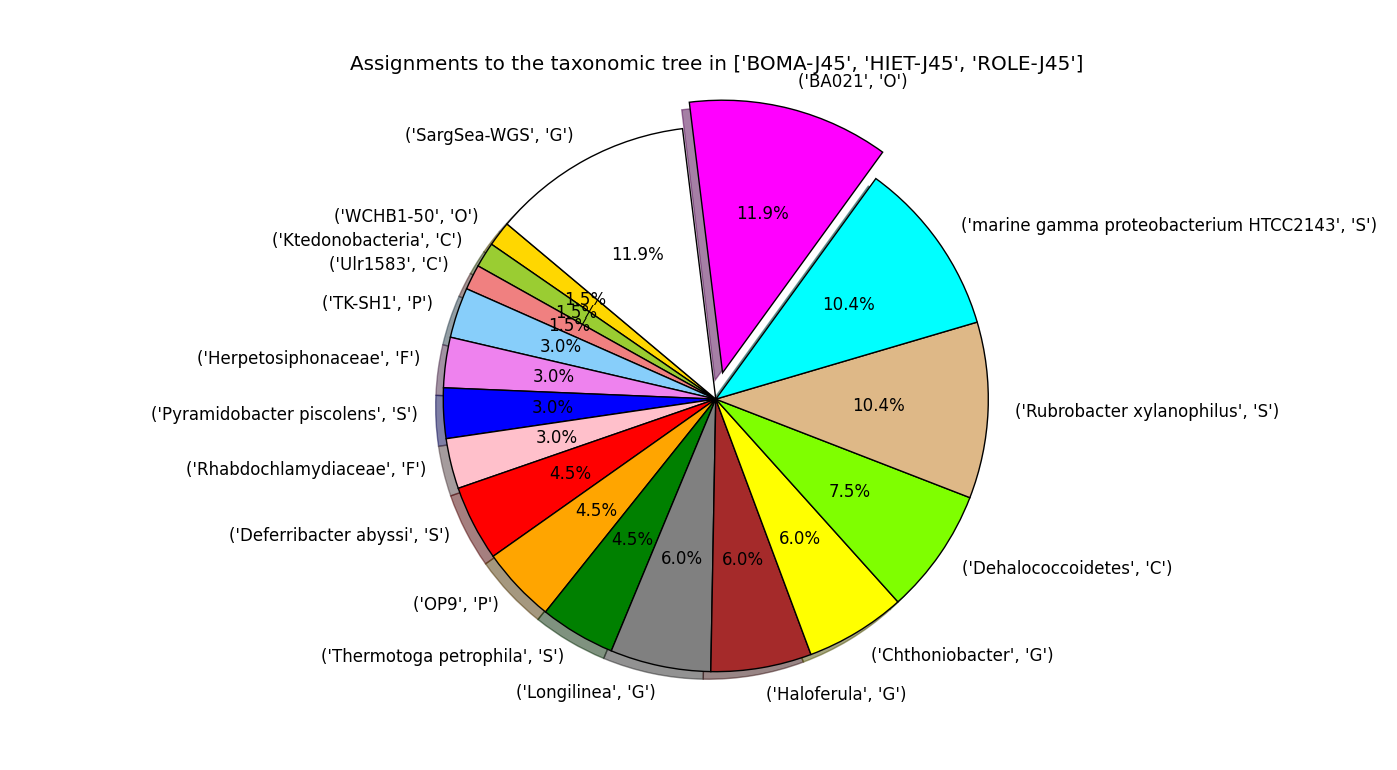
\includegraphics[scale=0.4]{illustrations/diversityDay451.png}
             \caption{Microbial Diversity Day=45, ATB-IV=1}
           \end{figure}

           \begin{figure}[H]
             \centering
             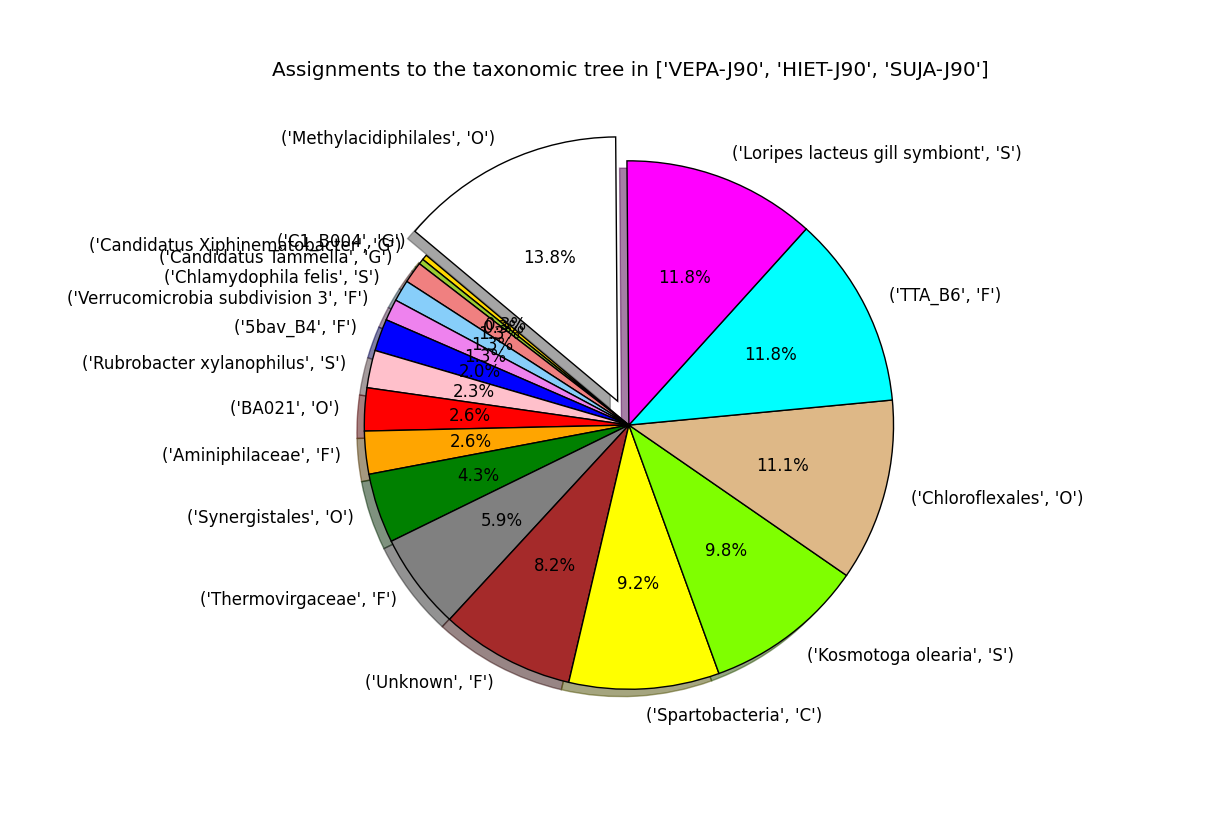
\includegraphics[scale=0.4]{illustrations/diversityDay901.png}
             \caption{Microbial Diversity Day=90, ATB-IV=1}
           \end{figure}
         \end{itemize}

\item \textsc{Comparison of the groups of samples at Day 90:}
       \textsc{Output of the statistical analyses (chapter 5.2.4):} $ATB-IV = 1$ and $ATB-IV = 0$ group still bear a significant difference.

     \begin{table}
       \caption{Results from \textsc{TaxoTree} for the comparison at Day 90, (*) for Day 0, (**) for Day 90}
       \begin{tabular}{|l|c|r|}
         \hline
         \textsc{Score} & \textsc{Result} & \textsc{Parameters}\\
         \hline
         Normalized Total Ratio & 0.92837592759 & ATB-IV=0,1 (*)\\
         \hline
         Normalized Total Ratio & 0.907051044683 & ATB-IV=0,1 (**)\\
         \hline
         Pattern Ratio & 9.46867603736 & ATB-IV=0,1 (*) \\
         \hline
         Pattern Ratio & 1.80113934679 & ATB-IV=0,1 (**) \\
         \hline
         Microbial Diversity & 0.0227222589896 & ATB-IV=0 (*)\\
         \hline
         Microbial Diversity & 0.0197440988308 & ATB-IV=1 (*)\\
         \hline
         Microbial Diversity & 0.0254798146923 & ATB-IV=0 (**)\\
         \hline
         Microbial Diversity & 0.0163247297595 & ATB-IV=1 (**)\\
         \hline
       \end{tabular}
     \end{table}

Although the microbial diversity is said to evolve the same way in both $ATB-IV = 1$ and $ATB-IV = 0$ groups, here the gap between the two diversity coefficient is deeper at Day 90 than at Day 0. We cannot tell if it is a natural variation, or an effect of the antibacterials. The difference between the samples increases according to the variation of \textsc{Pattern Ratio} coefficient, meaning microbial populations have evolved (under antibacterials?) between the two groups. Here, \textsc{Total Ratio} does not give any information.

\end{itemize}

\subsection{Overview and discussion}

\subsubsection{About the method}

The main issue with this program is thus to find relevant measures to characterize the samples. Since there is still many unknown things today about the biological mechanisms, we cannot be sure to get the best interpretation for these results. The algorithms below try to get rid of the \emph{a priori} hypotheses we could have over the biological mechanisms, that may have influence on the resulting scores.\\

This method is particularly naive, and tends to be close to the previous statistical analyses.\\

\subsubsection{About the numerical results}

Although being the most intuitive score, \textsc{Total Ratio} measure appears not to be really relevant here. This can be explained by the fact it does not take into account the proportions of assignments to nodes. As long as the two groups of samples owns a same node, it is considered as a common node, even though group $1$ might have many more reads assigned to this node than group $2$. On the opposite, \textsc{Pattern Ratio} seems justified by biology and gives consistent results.\\

Some of these results contradict the statistical results. We would need to test it on other databases to know who is right.\\

\chapter{Supervised learning}

The section just below will explain some important concepts, that will help to understand the second method, described in the following sections. 

\section{Machine Learning and supervised learning: the Naive Bayes classifier}

This section aims at explaining what \emph{Machine Learning} and \emph{supervised Learning} are, and at describing the \emph{Naive Bayes} classifier, and the \textsc{Youden's J coefficient} that will quantify the relevance of the classification.

\subsection{Machine Learning}

The last two approaches use Machine Learning type algorithms. \emph{Machine Learning} is a paradigm that automates the recognition of meaningful patterns in data \cite{SSS}, that is, the machine is technically able to sort the input according to certain criteria, without having the sorting explictly programmed.\\

For instance, it can be used to detect spam emails: the program searches throughout the emails keywords such as "fortune", "code bank", or "money". Then it evaluates (by computing the probability of having these keywords if the email is not a spam) whether the email should be discarded or not. If the probability of this email being a spam, with this number of keywords, is greater than the probability of this email being a regular email with these keywords, then the email is deleted. At the opposite, a 'regular' program would maybe need a threshold of number of occurrences above the one it discards the email. However, which value of threshold should we choose to be sure to keep (most of) our non-spam emails?\\

Along with the ability to deal with tremendously large files, \emph{Machine Learning} has nowadays become a quite common tool in bioinformatics \cite{Nikolski}. One of the ways to make the machine "learn" is called \emph{supervised learning}. 

\subsection{Supervised Learning}

\emph{Supervised learning} algorithms try to classify data into fixed labeled categories, basing their decision on prior experience with a training set of data, e.g. the algorithm from the spam example above. A set of emails comprising safe mails and spams (where the spam or non-spam nature of the emails is indicated) is given to the algorithm. It computes then (for instance) the probability of having occurrences of the words "fortune", "money", "love" in spam and non-spam emails. If the difference between the two probabilities is significant, it can help distinguish the unsafe mails out of the mailbox with the previous strategy.\\

One of the most used classifiers is the \emph{Naive Bayes} one.

\subsection{Naive Bayes Classifier}

Given $k$ (disjoint) classes of data $(C_{i})_{1 \le i \le k}$, a set of criteria $(F_{i})_{1 \le i \le m}$, and a datum $d$ to classify having $(F_{i} = x_{i})_{1 \le i \le m}$, the \emph{Naive Bayes classifier} computes $(P(C_{j} | F_{1} = x_{1},...,F_{m} = x_{m}))_{1 \le j \le k}$, that is, the probability of $d$ being in $C_{j}$ having these values of $(F_{i})_{1 \le i \le k}$. Then $d$ will belong to the class $C_{j}$ such as:\\

\begin{center}
$P(C_{j} | F_{1} = x_{1}, ..., F_{m} = x_{m}) = \max_{h \in \{ 1, ..., k \}}P(C_{h} | F_{1} = x_{1}, ... F_{m} = x_{m})$.\\
\end{center}

Since we do not know these probabilities, using Bayes' theorem, conditional probabilities can be rewritten this way (let $(F = x)$ be $(F_{1} = x_{1}, ..., F_{m} = x_{m})$):\\

\begin{center}
$P(C_{j} | F = x) = \frac{P(C_{j},F = x)}{P(F = x)}$\\ 
\end{center}

Using the chain rule, we can get:\\

\begin{center}
$P(C_{j},F_{1} = x_{1}, ..., F_{m} = x_{m})$\\ 
$= P(C_{j})P(F_{1} = x_{1} | C_{j})P(F_{2} = x_{2} | C_{j}, F_{1} = x_{1}) ... P(F_{m} = x_{m} | C_{j}, F_{1} = x_{1}, F_{2} = x_{2}, ..., F_{m-1} = x_{m-1})$\\
\end{center}

Under the assumption of independance between the $(F_{i})_{i}$, this can be rewritten as follows:\\

\begin{center}
$P(C_{j},F_{1} = x_{1}, ..., F_{m} = x_{m})$\\ 
$= P(C_{j})P(F_{1} = x_{1} | C_{j})P(F_{2} = x_{2} | C_{j}) ... P(F_{m} = x_{m} | C_{j})$\\
\end{center}

Eventually, the probability we are looking for is:\\

\begin{center}
$P(C_{j} | F = x) = \frac{P(C_{j})\prod{_{i = 1}^{m}}{P(F_{i} = x_{i} | C_{j})}}{P(F = x)}$\\ 
\end{center}

Later in this report, we use to compute $P(F_{i} = x_{i} | C_{j})$ the \emph{Bernouilli model}. This model has got a few drawbacks, but can be a good solution when relations between the $(F_{i})_{i}$ are unknown, and when the $(F_{i})_{i}$ can only have two (boolean) values.\\

If $p_{i}$ is the probability of $F_{i}$ being true, then:\\
\begin{center}
$P(F_{i} = x_{i} | C_{j}) = p_{i}^{x_{i}}(1 - p_{i})^{x_{i}}$
\end{center}

\subsection{Youden's J coefficient}

The measure used to quantify the relevance of the classification here will be \textsc{Youden's J coefficient} \cite{Youden}. Note that many other measures exist, such as \emph{F-measure} \cite{F-measure}, \emph{study of ROC space graph} \cite{IntroROC}, ... Since \emph{F-measure} raise certain issues \cite{FMproblems}, and knowing that \textsc{Youden's J coefficient} is often used for medical diagnosis, the latter has been here considered more helpful.\\

Some basics in statistics are required here. For a certain class \textsc{C}, we denote:
\begin{itemize}
\item \textsc{TP(C)} the True Positive data, that is the data that belongs to \textsc{C} and is assigned by the algorithm to \textsc{C}
\item \textsc{TN(C)} the True Negative data, not assigned to \textsc{C} and not belonging to \textsc{C}
\item \textsc{FN(C)} the False Negative data, not assigned to \textsc{C} and belonging to \textsc{C}
\item \textsc{FP(C)} the False Positive data, assigned to \textsc{C} and not belonging to \textsc{C}
\end{itemize}

\begin{figure}[H]
\centering
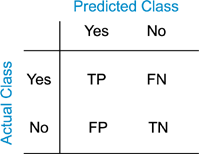
\includegraphics[scale=0.5]{illustrations/confusionmatrix.png}
\caption{\textsc{Confusion matrix} describing the four classes from gepsoft.com}
\end{figure}

Then the \textsc{Youden's J coefficient} for this class \textsc{C} is:\\

\begin{center}
$J(C) = \frac{TP(C)}{TP(C) + FN(C)} + \frac{TN(C)}{TN(C) + FP(C)} - 1$.\\
\end{center}

It uses respectively the \emph{recall}/\emph{sensitivity}\cite{F-measure} (the proportion of objects assigned to the right class among those assigned to \textsc{C}) and the \emph{precision}/\emph{specificity}\cite{F-measure} (the proportion of objects that do not belong to \textsc{C} among those not assigned to this class).\\

\begin{itemize}
\item When $J(C) = 1$, it means the classification is perfect (no \textsc{FN} and no \textsc{FP})
\item When $J(C) = 0$, it means the test does not do any better than a random classifier
\item When $J(C) = -1$, it means the test went all wrong (no \textsc{TP} and no \textsc{TN})
\end{itemize}

\section{Description of the method}

Second approach tries to answer problems (\textsc{A}) and (\textsc{B}). It uses a \emph{Naive Bayes Classifier}, which attempts to classify the samples/patients in one of the groups of values of metadata depending on their microbial populations.\\

\begin{enumerate}
\item The user is firstly asked to give the metadata \textsc{M} which will partition the set of samples, and the node population \textsc{N} to consider in the classification. It will set the number of classes, according to the different values for each metadatum of \textsc{M}.

\begin{figure}[H]
\centering
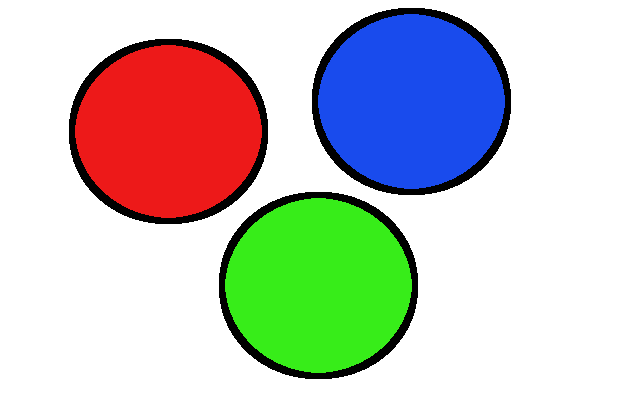
\includegraphics[scale=0.3]{illustrations/classessimples.png}
\caption{Let \textsc{M1} be a metadatum having values 0 (red), or 1 (green), or 2 (blue). Then there are three classes associated to \textsc{M1}.}
\end{figure}

\begin{figure}[H]
\centering
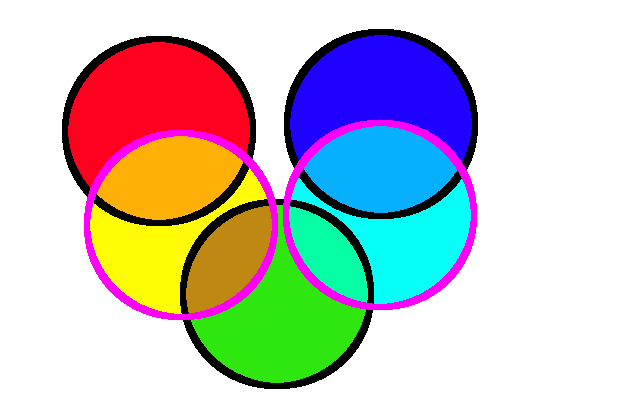
\includegraphics[scale=0.3]{illustrations/classescomplexes.png}
\caption{Let M2 be a metadatum having values 0 (yellow), or 1 (cyan). Then there are two classes associated to M2, that may intersect classes of M1. Thus there are four classes associated to M1 and M2 (classes do not take into account unknown values)}
\end{figure}

\item Then a random strict subset \textsc{R} of the initial set of samples is chosen to be the \emph{training set}. The size of this subset is chosen by the user. From this training set, the algorithm will compute an estimated probability of having a certain node for each node in \textsc{N} (corresponding to the $p_{i}$ described in the previous chapter), and also for each sample $s$ and for each node $n$, if $n$ appears in $s$ (this information is stored as a boolean value 0 or 1: with the previous notations, if $F_{i}$ is associated to node $n$, whether $F_{i} = 1 = x_{i}$ in sample $s$).

\item Hence for every sample in \textsc{R}, under the hypothesis of equiprobability of being in a certain class, the algorithm computes the probability of being in class \textsc{C} knowing the actual presence of the nodes in \textsc{N} for this sample, for each class \textsc{C}. 

\item The algorithm eventually assigns the sample to the class which maximizes this probability.

\end{enumerate}

The relevance of the resulting classification $f_{class}$ is quantified by the \textsc{Youden's J coefficient} $j_{f_{class}}$, pretty much like above. The best classification (that hightlights a significant correspondance between the values of the selected metadata and the microbial populations) is the classification such as, for all class $C$, $J_{f_{class}}(C)$ is the closest to 1.\\

In other words, if there are $k$ classes $(C_{i})_{1 \le i \le k}$,\\

\begin{center}
$k - \sum{_{i = 1}^{k}}{J_{f_{class}}(C_{i})}$ is minimum and non-negative.
\end{center}

\section{Implementation}

This has been implemented in \textsc{Python 2.9.7}. The program allows two operations, which answer to either \textsc{CL.C} or \textsc{CL.BCL}:\\

\begin{itemize}
\item The user chooses the sets \textsc{M} and \textsc{N} like above, and the program returns the \textsc{Youden’s J coefficient} associated to the resulting classification, giving a hint about a possible correspondance between \textsc{M} and \textsc{N}.
\item The user chooses two integers $s$ and $n$, the set \textsc{M}. Then the program randomly picks $s$ times $n$ distinct nodes in the taxonomic tree, and returns the set \textsc{N} of nodes of size $n$ which ensures the best classification (among the $s$ tries) for M. It may give a hint of a possible correspondance between \textsc{M} and the resulting set \textsc{N}.
\end{itemize}

The two main issues with the \textsc{K-Means} algorithm is to choose $k$ and the initialization of the clusters. Fortunately, our method solves these problems since $k$ is the number of metadata classes associated to the user-selected metadata, and each cluster is initialized with a sample having the correct values of metadata associated to this cluster.\\

To deal with multiple metadata classes (see the example above), multi-dimensional lists have been implemented (see annex).\\

The overall worst case time complexity for a classifiation is roughly in O($n_{samples}^{2} \times n_{taxo-nodes}^{2} \times n_{values}$) (see annex for more details).\\

(Still in progress) code can be found at:\\ \emph{https://github.com/kuredatan/taxoclassifier}.

\section{Results}

\subsection{Tests}

%todo

\subsection{Overview and discussion}

\subsubsection{About the method}

Although the algorithm classifies samples not by focusing on specific characteristics of node population, but by directly comparing the microbial populations (which is theoretically better than the previous program), we still have to do \emph{a priori} hypotheses on the set of samples.\\

Firstly, we suppose the equiprobability of being in a random class, that is, equiprobability of having a certain value for the selected metadatum. However, not only does it strongly depend on the values of other metadata, but it would even be sometimes completely wrong according to the metadatum considered. In our database for instance, $ATB-IV = 1$ or $ATB-Os = 1$ imply $ATB-IV-Os = 1$: $ATB-IV = 1$ means patient has been treated with antibacterials by intraveinous injections (\emph{IV}), $ATB-Os = 1$ means patient has been treated with antibacterials \emph{per os}, and $ATB-IV-Os = 1$ means patient has been treated with antibacterials either \emph{per os} or \emph{IV}. Unfortunately, since we do not know the exact relationship between the different metadata (e.g. does the treatment really affect the quality of life of the patient?), we cannot fix this issue.\\

Same goes for the hypothesis of independance between the probabilities of having a certain node, that is at core of the Bayes conditional model. Biologically speaking, we can wonder if having a certain species of bacteria may prevent another species to develop itself in the gut.\\

Secondly, the size and the content of the starting set for the classification given by the \emph{Naive Bayes Classifier} is of paramount importance. Prior probabilities of having a certain node are computed from this starting set by default (because assuming equiprobability would lead to contradictions, since we know antibacterials for instance do affect the microbial population). If the starting set is badly chosen, some nodes might not have matched any read in the starting group of samples, and thus the probability of having such a node is theoretically zero. Then the Bernouilli model would always return zero for a probability of being in a certain class, if this node is selected.\\

We thus let the user choose themselves the size of the starting set, provided the total size of the set of samples to classify.\\

A solution to this problem is to use the \emph{Bayesian average} \cite{BayesianRating}, that is, if the probability $p_{n}$ of having the node $n$ computed from the starting set $S_{start}$ and:

\begin{itemize}
\item $N_{n}$ be the number of samples having node $n$ among the samples in the starting set
\item Boolean variable $x_{i,j} = 1$ iff node $j$ is matched in sample $i$ (else $x_{i,j} = 0$)
\item $M_{n} = \frac{N_{n}}{|S_{start}|}$ 
\item $v_{n} = \sqrt{\sum{_{i=1}^{S_{start}}}{(x_{i,n} - M_{n})^{2}}}$
\item $C_{n} = \frac{|S_{start}|}{v_{n} + 1}$
\item $m_{n} = \frac{C_{n}}{|S_{start}|}$
\end{itemize}

\begin{center}
Then $p_{n} = \frac{C_{n}.m_{n} + N_{n}}{C_{n} + |S_{start}|}$\\
\end{center}

The idea of \emph{Bayesian average} is not to fully rely on the samples of the starting set to compute the probabilities of having a certain node. $C_{n}$ will be a coefficient denoting how much confident we are in the probabilities given by the starting set. The more we believe the probabilities will be distributed on the whole set of samples the same way they do in the starting set, the larger is $C_{n}$. This is quantified by the variation of values in the starting set: if most of the samples have matched this node -that is, variation is low- it is likely that all samples may actually own this node.\\

Note that the maximum value of $C_{n}$ is $|S_{start}|$. Having $C_{n} = |S_{start}|$ (that is $v_{n} = 0$), would mean we completely trust the starting set (replacing $C_{n}$ in the formula above leads to $p_{n} = \frac{|S_{start}| + N}{2.|S_{start}|}$), whereas $C_{n} = 0$ gives $p_{n} = \frac{N_{n}}{|S_{start}|}$, that is, we consider the non-amplified values of probabilities from the starting set.\\

For instance, if node $n$ matches in $5$ samples out of $17$, having $C_{n} = 0$ would give $p_{n} = \frac{5}{17} \simeq 0.29$, while having $C_{n} = |S_{start}|$ gives $p_{n} = \frac{17 + 5}{2 \times 17} \simeq 0.65 $. If node $n$ does not match in any of the $17$ samples, then for $C_{n} = \frac{|S_{start}|}{2}$, $p_{n} = \frac{|S_{start}|}{4 \times |S_{start}|} = \frac{1}{4} = 0.25$.\\

\subsubsection{About the numerical results}

%todo

\chapter{Non-supervised learning}

The following sections will introduce some useful concepts and notations, that will help to understand the third method described at the end of this chapter.

\section{Machine Learning and non-supervised learning: the K-Means algorithm}

This section explains what \emph{non-supervised learning} is in \emph{Machine Learning}, and present one of the most common tool in this category, which is the \emph{K-Means algorithm}.

\subsection{Non-Supervised Learning}

Another broad category in \emph{Machine Learning} is \emph{non-supervised learning}: unlike \emph{supervised learning}, the different classes to which belong the data are not known at first. Provided the set of elements, the algorithm has to distinguish by itself several different classes according to the similarity between the pieces of data from the initial set. This is why one of the most common approach for \emph{non-supervised learning} is \emph{clustering}.

\subsection{Clustering}

Given a certain distance, \emph{clustering} is the task of gathering objects into disjoint clusters, such as the resulting clusters maximize the proximity (in terms of the chosen distance) between elements of a same cluster, and maximize the distance between objects of different clusters.

\subsection{K-Means Algorithm} 

Although the problem of partitionning $n$ elements into $k$ clusters \cite{PartitionIsNPhard} is \textsc{NP-hard}\cite{NPhard} (see the note in bibliography for a definition of \textsc{NP-hardness}), the \emph{K-Means algorithm} \cite{KMeans} is a rather efficient clustering algorithm. After choosing an integer $k$ that will be the estimated number of clusters, the user initializes each cluster with one of the elements of the set. Then, for each non-clustered object, the algorithm computes the distance from this object to the mean of every cluster (in our implementation, it is the sample that minimizes the sum of all distances to the other samples in the same cluster), and assigns the object to the closest cluster. Then it updates the mean of this cluster, and iterates the last two steps until convergence of the solution. For more detailed explanation, see \cite{KMeans}.

\section{Definitions}

Before starting to describe the method, here are some helpful notations (adapted from \cite{Tango1}):\\

\subsection{Notations}

Knowing \textsc{T} is the whole taxonomic tree, for a certain read $i$, let $M_{i}$ be the set of matched leaves for this read, and $T_{i}$ the subtree of \textsc{T} rooted at the \textsc{LCA} (see above for the definition of \textsc{LCA}) of the nodes in $M_{i}$. Let $L_{i}$ be the set of leaves of $T_{i}$, and $N_{i}$ be such as $L_{i} = M_{i} \sqcup N_{i}$.

\begin{figure}[H]
\centering
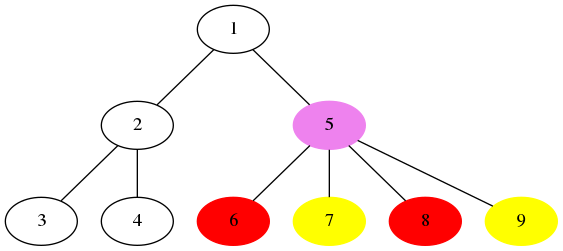
\includegraphics[scale=0.3]{illustrations/timili.png}
\caption{Let T be this tree. Then for the set of red nodes, the subtree associated is rooted at the violet node, and the total set of leaves for this subtree is the set of yellow and red nodes.}
\end{figure}

\subsection{Distances}

Let us define two distances $d_{matched}$ and $d_{consensus}$ over pairs of reads ($R_{i},R_{j}$) for the clustering:
       \begin{itemize} 
       \item \begin{center} $d_{matched}(R_{i},R_{j}) = |M_{i}| + |M_{j}| - 2*|M_{i} \cap M_{j}|$. \end{center}\\ 

It is quite easy to check that $d_{matched}$ is indeed a distance: $d_{matched}$ is symmetric, satisfies the triangle inequality, is non-negative, and $d_{matched}(i,j)$ equals to zero iff $R_{i} = R_{j}$ (The unique relevant equality relation between reads here is the equality between the respective sets of matched nodes, because nobody can know to which node the read should truly be assigned).
       \item Having a fixed parameter $q \in [0,1]$,\\
\begin{center}
$d_{consensus}(R_{i},R_{j}) = |L_{i}| + |L_{j}| - q*(|N_{i}\cap M_{j}| + |N_{j} \cap M_{i}|) - |M_{i} \cap M_{j}|$.\\
\end{center}

It is also easy to check here that $d_{consensus}$ is a distance. This distance corresponds to search a consensus taxonomic tree between the trees induced by the set of nodes matched by the reads \cite{Consensus}.\\

When $q = 0$, we consider a \emph{strict} consensus tree, only keeping leaves matched in both reads.\\
When $q = 1$, we consider a tree having leaves that are matched in at least one of the two reads.

\begin{figure}[H]
\centering
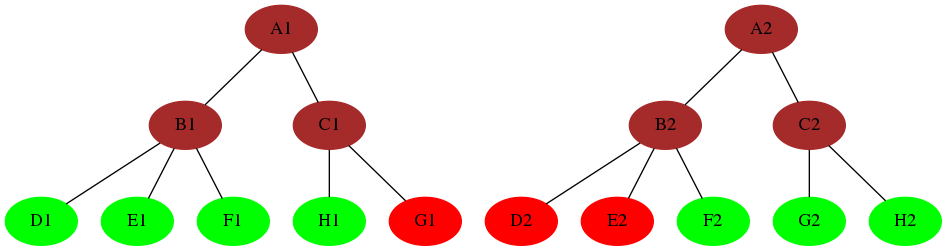
\includegraphics[scale=0.5]{illustrations/distance2.png}
\caption{Let us consider the cyan/blue and orange/red trees (blue and red nodes being the ones matched, the yellow one being matched by the orange tree and not by the blue tree, the two violet nodes are matched in both trees). When $q = 0$, $d_{consensus}(t_{1},t_{2})$ applied to these trees $t_{1}$ and $t_{2}$ is equal to $(2 + 4) - 0 \times (1 + 0) - 2 = 4$. When $q = 1$, $d_{consensus}(t_{1},t_{2})$ is equal to $(2 + 4) - 1 \times (1 + 0) - 2 = 3$}
\end{figure}

       \end{itemize}
\item These distances can easily be extended to samples: if $Reads_{k}$ is the set of reads for sample $S_{k}$,\\
\begin{center}
$d_{consensus}(S_{k},S_{l}) = \sum{r_{k} \in Reads_{k}}{\sum{r_{l} \in Reads_{l}}{d_{consensus}(r_{k},r_{l})}}$.
\end{center} 

Same goes for $d_{matched}$.

\section{Description of the method}

The third approach tries to answer problem (\textsc{A}). It compares trees induced by samples before assignment of reads, and avoids providing \emph{a priori} hypotheses on the probabilities of being in a certain class of metadata values, or of having a certain node. The number $k$ of clusters used in the \textsc{K-Means} algorithm is thus the number of vectors of metadata that can be obtained.\\

We use the very same definition of classes of metadata as in the second method.

\begin{itemize}
\item Firstly the set of samples is clustered into $k$ clusters using $d_{matched}$ distance. 
\item For every cluster, the most remote elements are deleted from the cluster. In our implementation, the points which sum of all distances to other samples of the same cluster is above the value of the third quartile (of the list of such distances) are the ones discarded.
\item Then the union of the remaining elements in all clusters is clustered again into $k$ clusters using $d_{consensus}$ distance.
\end{itemize}

The clusters resulting from the second clustering are then compared to the clusters obtained by directly looking at the values of metadata in samples. If the two groups of clusters are alike (this is quantified by a special distance), this could mean there exists a correspondance between the selected metadata and the microbial populations. The program also returns the bacteria in common for samples in a same cluster.\\

\section{Implementation}

The whole pipeline has been implemented in \textsc{Python 2.9.7}, and allows to draw and see the clusters in a DOT file.\\

The worst case time complexity is O($n_{samples}^{2} \times (n_{samples} \times n_{paths} \times n_{taxo-nodes} + n_{taxo-nodes}^{2}) \times n_{samples}^{2}$) (see annex for details).\\

(Still in progress) code can be seen at: \\\emph{https://github.com/kuredatan/taxocluster}.

\section{Results}

\subsection{Tests}

%todo

\subsection{Overview and discussion}

\subsubsection{About the method}

However, the main issue with this method is that, unlike the first \emph{Machine Learning} approach, it does not give the nodes that really discriminate the samples. We can only get access to the list of common bacteria for samples in a same cluster. One solution would be to post-process the clusters with a \textsc{PCA} (\emph{Principal Component Analysis}) method \cite{PCA}, or to test this pipeline with another clustering algorithm (different from \emph{K-Means}).

\subsubsection{About the numerical results}

%todo

\newpage

\chapter{Comparison of the three approaches}

The third algorithm is thought to be theoretically best, as it would fix the issues in the first two methods. In terms of worst case time complexity, knowing the actual values for each variable in our test database, it is also one of the best ones:\\

    \begin{table}
      \caption{Complexity for each method}
      \begin{tabular}{|l|c|r|}
        \hline
        \textsc{Method} & \textsc{Theoretical complexity} \\
        \hline
        Statistics & O($n_{taxo-nodes}^{2} \times n_{samples}^{3}$)\\
        \hline
        Supervised learning & O($n_{samples}^{2} \times n_{taxo-nodes}^{2} \times n_{values}$)\\
        \hline
        Non-supervised learning & O($n_{samples}^{2} \times n_{taxo-nodes}\times (n_{samples} \times n_{paths})$)\\
        \hline
      \end{tabular}
    \end{table}

Nevertheless, to fully validate the results from the algorithms, we should get access to several other databases, and compare them to the output of statistical methods. We unfortunately could not use any other database to perform these necessary tests. Furthermore, the consistency of results greatly depends on the operations applied to input data (have the numeric results been normalized prior to the algorithm? Have all raw material for samples been collected the same way, following a same standard procedure? Has each assignment of read to nodes been performed under the same parameters? ...). And, last but not least, the final interpretation of the results cannot still be taken into account without the practitionner's approval.

\chapter{Outlook}

During this internship, we suggested three methods to analyse data from sequencing. We also have implemented a class of multi-dimensional lists, and an rather efficient algorithm to reconstruct taxonomic trees from the list of paths to the leaves.\\

The use of algorithms from \emph{Machine Learning} in metagenomics is not so new \cite{Nikolski}, but is used here to draw parallels between metadata, that are processed most of the time today by statistical analyses, and trees, that are one of the most important parts of algorithmics.\\

On the one hand, a quite large number of comparison problems over labeled ordered trees are \textsc{NP-complete}, for instance tree inclusion \cite{TreeInclusion}. What makes possible efficient algorithms is that the relevant comparison over trees here mainly focuses on the set of leaves for each tree. However, the time complexity of the last two methods should still be improved.\\

On the other hand, it would be interesting to test these algorithms on other databases than the one of cystic fibrosis-afflicted patients.

\newpage

\bibliographystyle{plain}
\bibliography{rapport.bib}

\newpage

\appendix

\chapter*{Annex}

Here are gathered details about the physical limits of our computer for testing, detailed complexity function by function for each of the three methods described above, different algorithms to reconstruct a taxonomic tree as well as the implementation of multi-dimensional lists used in two out of the three methods.

\chapter{Physical characteristics of the testing computer}

\begin{itemize}
\item \uline{Processor:} Intel Core i3-3227U 3rd generation
\item \uline{Clock speed:} 1.90 GHz
\item \uline{3rd level cache:} 3 Mo
\item \uline{Hard Disk:} 1 To, rotation speed: 5,400 r/min
\item \uline{RAM:} 6 Go, max: 16 Mo, DDR3 1,600 MHz
\end{itemize}

\chapter{Complexity}

This chapter give details about the complexity of each method, per function and for the whole pipeline.

\section{Worst case complexity for the first approach (TaxoTree)}

Let $n_{samples}$ be the total number of available samples (in our test database, $n_{samples} = 47$), and $n_{taxo-nodes}$ the number of nodes in the taxonomic tree ($n_{taxo-nodes} = 9,000$).

\subsection{Per function}

\begin{itemize}
\item \textsc{Total Ratio:} See functions \emph{misc/inSample}, \emph{misc/takeNodesInTree}, \emph{totalRatio/compute} and \emph{totalRatio/countAssignmentsInCommon}.\\

\uline{inSample}: @sampleNameList (the list of user-selected samples) can be as large as the whole list of samples: O($n_{samples}$).\\

\uline{takeNodesInTree}: This procedure does a top-down search in the taxonomic tree, and executes \emph{inSample} for each list of assignments, that is, for each node of the taxonomic tree: O($n_{taxo-nodes} \times n_{samples}$).\\

\uline{compute}: \emph{compute} executes twice \emph{takeNodesInTree}. The member function \emph{mem} is in O($n_{taxo-nodes}$). In the worst case where the two user-selected lists are the same, the following operations are in O($size of the first subforest$) = O($n_{taxo-nodes}$). So \emph{compute} is in O($n_{taxo-nodes} \times n_{samples}$).\\

\uline{countAssignmentsInCommon}: It can easily be seen that \emph{countAssignmentsInCommon} is in O($n_{taxo-nodes}.n_{samples}^{2}$).\\

The overall complexity is thus O($n_{taxo-nodes} \times n_{samples}^{2}$). The most costly part is \emph{countAssignmentsInCommon}.

\item \textsc{Pattern Ratio:} See functions in \emph{patternRatio} and \emph{taxoTree} modules.

\uline{TaxoTree.search}: The procedure does a top-down search in the tree for the node in argument: O($n_{taxo-nodes}$).\\

\uline{misc/mergeList}: The procedure takes two lists of length $n$ and $m$, sorts both of them and then merge the two lists without duplicates (assuming there is no duplicate in the two lists): O($nlog(n) + mlog(m)$).\\

\uline{misc/trimList}: This procedure takes two lists of length $n$ and $m$, and deletes from the first list elements that belongs to the second one. It sorts both of the lists, and then considers in linear time the elements of the two lists. Thus the time complexity is O($nlog(n) + mlog(m)$).\\

\uline{enumerateCommonPatterns}: This function uses \emph{takeNodesInTree} and considers every node from the tree induced by the user-selected set of samples as a potential starting point for a pattern, and then tries to spread the pattern to the node's children, if it is possible (that is, if the child is matched at least in one of the samples in the user-selected list: the test is in O($n_{samples}$)). The two lists of assignments to this node are merged using \emph{mergeList} procedure: O($n_{samples}log(n_{samples})$). Final time complexity is thus O($n_{taxo-nodes} \times n_{samples} + n_{taxo-nodes}^{2} \times (n_{samples} + n_{samples}log(n_{samples}))$) = O($n_{taxo-nodes}^{2} \times n_{samples}log(n_{samples})$).\\

\uline{enumerateSpecificPatterns}: This function takes into argument the two user-selected lists of samples, uses \emph{trimList} procedure to have disjoint lists (such as one pattern of the first list does not belong to the second list, and the other way around), and then executes pretty much the same procedure as \emph{enumerateCommonPatterns}. Thus the time complexity is O($n_{taxo-nodes}^{2} \times n_{samples} + n_{samples}log(n_{samples})$).\\

\uline{patternRatio}: This function counts the number of assignments for all (common or specific) patterns. These patterns are disjoint, by construction, so in the worst case, it counts assignments for every node of the taxonomic tree: O($n_{taxo-nodes}$).\\

Henceforth using the \textsc{Pattern Ratio} procedure is\\
in O($n_{taxo-nodes}^{2} \times n_{samples}log(n_{samples})$) time.

\item \textsc{Microbial Diversity:} See \emph{computeDiversityCoefficient} function in \emph{diversityCoefficient} modules.

\uline{computeDiversityCoefficient}: This procedure uses \emph{takeNodesInTree} (see the chapter above). It considers every node in the tree induced by the user-selected list of samples, and counts the total number of assignments to this node in samples belonging to the list (O($n_{samples}$) if the list of samples contains all available samples).\\

Thus the overall complexity is O($n_{taxo-nodes} \times n_{samples}$).

\end{itemize}

\subsection{Overall complexity}

Therefore, to compute the distance described above for every pair of samples ($\frac{n_{samples}(n_{samples} - 1)}{2}$ pairs, distance being symmetric):\\

The time complexity is roughly in O($n_{taxo-nodes}^{2} \times n_{samples}^{3}$).

\section{Worst case complexity for second approach (TaxoClassifier)}

Without loss of generality, complexity will evaluated without multi-dimensional lists, since one metadatum can have an arbitrary number of different values.\\

Let $n_{samples}$ be the total number of available samples (in our test database, $n_{samples} = 47$), and $n_{taxo-nodes}$ the number of nodes in the taxonomic tree ($n_{taxo-nodes} = 9,000$). Let $n_{values}$ the maximum number of effective values in the information matrix that a metadatum can have, that is, the maximum number of classes -in our test database, $n_{values}$ is bounded by $10$, metadatum $Sample$ excepted. Let eventually $n_{metadata}$ the total number of metadata ($n_{metadata} = 21$). 

\subsection{Per function}

\begin{itemize}
\item \textsc{Training:} See functions in \emph{training} module.\\

\uline{computeClasses}: See \emph{misc/partitionSampleByMetadatumValue}: O($n_{samples}log(n_{samples}) + n_{metadata}$).\\

\uline{selectTrainingSample}: O($n_{samples}$) (Reservoir Sampling R algorithm).\\

\uline{assignClass}: O($n_{samples}^{2} \times n_{values}$).\\

\uline{getPriorProbability}: O($n_{samples}^{2} \times n_{taxo-nodes}^{2}$).\\

The overall complexity is hence O($n_{samples}^{2} \times n_{taxo-nodes}^{2} + n_{samples}^{2} \times n_{values} + n_{metadata}$)\\
 = O($n_{samples}^{2} \times n_{taxo-nodes}^{2}$). \\

\item \textsc{Classification:} See functions in \emph{classifier} module.\\

\uline{probabilityKnowingClass}: O($n_{taxo-nodes} \times n_{samples} \times n_{taxo-nodes}$) = O($n_{taxo-nodes}^{2} \times n_{samples}$).\\

\uline{bayesCalculus}: The most costly part is the call to \uline{probabilityKnowingClass}: O($n_{taxo-nodes}^{2} \times n_{samples}$). \\

\uline{classifyIt}: with the call to \uline{trainingPart}: O($n_{samples}^{2} \times n_{taxo-nodes}^{2} \times n_{values}$).\\

\item \textsc{Computation of Youden's J coefficient:} See \emph{countYouden} function in \emph{youden} module.

The whole set of classes contains at maximum the $n_{samples}$ samples. Thus the loop over the classes is in fact a loop over the set of samples. Then the overall time complexity is O($n_{samples}^{2} + n_{values}$).\\

\end{itemize}

\subsection{Overall complexity}

The worst case time complexity is roughly in O($n_{samples}^{2} \times n_{taxo-nodes}^{2} \times n_{values}$).

\section{Worst case complexity for third approach (TaxoCluster)}

Same notations as in previous chapter are used here. The most costly part in the clustering is the call to \textsc{K-means}, the computation of the two distance matrix, and the comparison between clusters.\\

\subsection{Per function}

\begin{itemize}
\item \textsc{Distances:} Between two given samples:\\

\begin{itemize}
\item \textsc{Distance 1:} The maximum length of the list of matching nodes is $n_{taxo-nodes}$ (lists of matching nodes are stored in a dictionary). Thus time complexity is in O($n_{taxo-nodes}^{2}$).\\

Thus the computation of the whole distance matrix has got a worst case time complexity of O($n_{taxo-nodes}^{2} \times n_{samples}^{2}$).

\item \textsc{Distance 2:} The computation of the \textsc{LCA} of a list of nodes of length $m$ ($m$ is bounded by $n_{samples}$) is in O($m \times n_{paths} \times l_{path}$) (see \emph{misc/taxoLCA}). The search of subtrees is in O($n_{taxo-nodes}$) (see above), as well as the call to \emph{TaxoTree.leaves} that counts leaves of the tree. The final loop is in O($n_{taxo-nodes}$).\\

Thus the computation of the whole distance matrix has got a worst case time complexity of O($n_{samples}^{2} (n_{samples} \times n_{paths} \times l_{path} + n_{taxo-nodes})$).

\end{itemize}

\item \textsc{K-means:} O($(n_{samples} - n_{values}) \times n_{values} \times n_{iterations}$) where $n_{iterations}$ is the number of needed iterations until convergence (30).

\item \textsc{Cluster comparison:} For two given clusters (maximum sum of both lengths being $n_{samples}$: thus maximum value of the product of the lengths is $(\frac{n_{samples}}{2})^{2}$):

\uline{compareCluster}: O($n_{samples}^{2}$)\\

\uline{compareCenters}: for two given clusters: O($1$) (storing distances between samples in a dictionary).\\

\end{itemize}

\subsection{Overall complexity}

Thus the worst case time complexity is\\
O($(n_{samples} - n_{values}) \times n_{values} \times n_{iterations} + n_{samples}^{2} \times n_{values}^{2} + n_{samples}^{2} (n_{samples} \times n_{paths} \times l_{path} + n_{taxo-nodes}) + n_{taxo-nodes}^{2} \times n_{samples}^{2}$)\\
= O($n_{samples}^{2} \times (n_{samples} \times n_{paths} \times n_{taxo-nodes} + n_{taxo-nodes}^{2} \tmes n_{samples}^{2})$).

\chapter{Construction of taxonomic trees}

\section{State-of-the-art and input}

There are of course many algorithms to construct a taxonomic tree, often starting from a distance matrix between the \emph{taxa} (plural of \emph{taxon}, that is, nodes of the phylogenetic tree); for instance, \textsc{Neighbor Joining} \cite{NeighborJoining}, or \\ \textsc{Unweighted/Weighted Pair Group Method with Arithmetic\\ Mean} \cite{UMPGA}. However, here we have already got the whole taxonomic tree and the phylogenetic relation between the \emph{taxa}.\\

Provided a list of paths \emph{paths} from the root to every leaf of the phylogenetic tree, we thus need an efficient algorithm to construct the tree, which must grant easy (i.e. as cheap as possible) access to the list of assignments to node, to the children and also to the phylogeny of the node (the so-called "lineage"). It should also provide labelling of the nodes by an integer identifier. Since we could not find an article having dealt with this subject (trace analysis do use trees, but since we are interested in a very special sort of tree (taxonomic trees), it would be a bit off topic here), we had to design a customized algorithm.\\

Let $n_{taxo-nodes}$ be the number of the nodes in the taxonomic tree (in our test database, $n_{taxo-nodes} = 9,000$), $n_{samples}$ the number of samples ($n_{samples} = 47$), and $n_{paths}$ the number of paths from the root to every leaf (as it is a tree, this number is as well the number of leaves in the tree, that is $n_{paths} \simeq 8,000$). Let also $l_{path}$ be the maximum length between the root and a leaf (that is the number of ranks: in our test database, $l_{paths} = 8$), and $n_{metadata}$ the number of metadata ($n_{metadata} = 21$).

We present three methods in chronological order of design:
\begin{itemize}
\item The first one is a top-down construction, where we go through every path from \emph{root} to a leaf, and construct the missing nodes.
\item Unlike the method above, the second one is a bottom-up construction, where for each taxonomic rank (from S to R, that is from the most accurate to the most broad rank), we gather siblings (that is nodes with a same father) and construct the corresponding trees until having the tree rooted at \emph{root}.
\item The third one is an improvement of the second method. The first two methods are quite time-consuming, and this one succeeds in being the fastest of the three. Preprocess is applied to the nodes to precompute the groups of siblings and the father node associated, using hash tables.
\end{itemize}

\section{A naive top-down construction}

The method is to consider one by one every path from \emph{paths} and to create the branch of nodes when the algorithm finds a uncreated node while following the path (Algorithm 1).\\

\textsc{INPUT:} \emph{paths} the list of paths from the root to every leaf of the tree, \emph{root} the root of the empty taxonomic tree.\\

\textsc{OUTPUT:} The corresponding taxonomic tree rooted at \emph{root}.\\

\begin{algorithm}
\caption{The naive top-down construction}
\begin{algorithmic}
\FOR{path in \emph{paths}}
\STATE $currNode \leftarrow \emph{root}$
\STATE $currLineage \leftarrow [ (\emph{root}.name, \emph{root}.rank) ]$
\STATE $currChildren \leftarrow \emph{root}.children$
\STATE $currPath \leftarrow \emph{paths}.tail()$
\WHILE{currPath is non-empty}
\STATE $name,rank \leftarrow currPath.head()$
\STATE $nextNode \leftarrow$ currNode's child which name, rank are $name$, $rank$
\IF{$nextNode \neq NONE$}
\STATE $currNode \leftarrow nextNode$ 
\STATE $currLineage \leftarrow append(currLineage,[(currNode.name,currNode.rank)])$
\STATE $currChildren \leftarrow currNode.children$
\ELSE
\STATE $sampleList \leftarrow$ the list of assignments associated to (name,rank)
\STATE Create the node $node$ associated to name,rank and add it to the list of children of currNode
\STATE $currNode \leftarrow node$
\STATE $currLineage \leftarrow append(currLineage,[(currNode.name,currNode.rank)]) $
\WHILE{currPath is non-empty}
\STATE $name,rank \leftarrow currPath.head()$
\STATE $sampleList \leftarrow$ the list of assignments associated to (name,rank)
\STATE Create the node $node$ associated to name,rank and add it to the list of children of currNode
\STATE $currNode \leftarrow node$
\STATE $currLineage \leftarrow append(currLineage,[(currNode.name,currNode.rank)]) $
\ENDWHILE
\ENDIF
\ENDWHILE
\ENDFOR
\RETURN{\emph{root}}
\end{algorithmic}
\end{algorithm}

Worst case time complexity: O($l_{path}.n_{paths}.n_{metadata}.n_{samples}$). It takes approximately 2 hours on our computer to construct the tree associated to the parsed \emph{paths} list.

\section{A naive bottom-up construction}

The previous method can be used for any type of tree. However, taxonomic trees are special indeed. Their height is bounded by the number of ranks in the phylogeny, and there are much more leaves than internal nodes. The following algorithm tries to take advantage of these two characteristics (Algorithm 2): it considers the nodes in decreasing rank (in terms of taxonomic accuracy), then look for each of them their children, create the tree associated to the nodes, and iterates this process until all the nodes had been turned into trees. It eventually returns the tree rooted at \emph{root}.\\

\textsc{INPUT:} \emph{paths} the list of paths from the root to every leaf of the tree, \emph{root} the root of the empty taxonomic tree, \emph{ranks} the array of ranks in the phylogeny in order of decreasing taxonomic precision (S, then G, then F, O, C, P, ...), and \emph{nodesList} the list of nodes in the phylogenetic tree.\\

\textsc{OUTPUT:} The corresponding taxonomic tree rooted at \emph{root}.\\

\begin{algorithm}
\caption{The naive bottom-up construction}
\begin{algorithmic}
\STATE $currConstructedTrees \leftarrow$ []
\STATE $numberRanks \leftarrow$ ranks.length()
\FOR{i in { 1, ..., numberRanks }}
\STATE $currNodesToProcess \leftarrow$ the list of nodes having rank \emph{ranks}[i]\\ //look at each node in \emph{nodesList}, push it to currNodesToProcess iff its rank equals ranks[i]
\STATE $potentialChildrenTrees \leftarrow$ currConstructedTrees
\FOR{node in currNodesToProcess}
\STATE $currSampleList \leftarrow$ the list of assignments associated to node $node$
\STATE $currLineage \leftarrow$ the phylogeny of the node $node$
\STATE $currChildrenNameRank \leftarrow$ the list of (name,rank) pairs of node's children
\STATE $currChildren \leftarrow$ []
\STATE $currNotChildren \leftarrow$ []
\WHILE{potentialChildrenTrees is non-empty}
\STATE $currTree \leftarrow$ potentialChildrenTrees.head()
\IF{currTree belongs to currChildrenNameRank}
\STATE $currChildren \leftarrow$ append(currChildren,currTree)
\ELSE
\STATE $currNotChildren \leftarrow$ append(currNotChildren,currTree)
\ENDIF
\STATE $currConstructedTrees \leftarrow$ currNotChildren
\STATE $tree \leftarrow$ create the tree associated to node 
\STATE $currConstructedTrees \leftarrow$ append(currConstructedTrees,tree)
\ENDWHILE
\ENDFOR
\ENDFOR
\RETURN{currConstructedTrees.head()}
\end{algorithmic}
\end{algorithm}

Worst case time complexity: O($n_{taxo-nodes}.(n_{samples}.n_{metadata} + n_{paths}.l_{path} + n_{paths}^{2})$). Please note that the number of leaves bounds the width/maximum degree of the taxonomic tree. The number of ranks can be bounded by a constant integer (for instance, $10$). It thus takes approximately $10$ hours (!) on our computer to construct the taxonomic tree.\\

\section{A less naive bottom-up construction}

The previous bottom-up algorithm has got a really bad time complexity, for it must recompute each time the lineage and the lists of assignments. This following method fixes this issue, by precomputing the lineage and the other phylogenetic relations (Algorithm 3) and then using it to get the whole taxonomic tree (Algorithm 4). \\

\textsc{A few definitions:}
\begin{itemize}
\item A \textsc{brotherhood} is a list of nodes having the same father in the taxonomic tree. In case of a taxonomic tree, every node of the brotherhood has got the very same rank.
\item \textsc{hashBrotherList} is a list such as \emph{hashBrotherList}[i] = (n,m) means the (i+1)th node in the list of nodes sorted by ranks belongs to the (m+1)th brotherhood of rank number (n+1) (in order of decreasing rank).
\item \textsc{hashFatherList} is a list such as \emph{hashFatherList}[i] = (n,m) means the (i+1)th node is the father of the nodes of the (m+1)th brotherhood of rank number (n+1) (in order of decreasing rank). Unlike in \emph{hashBrotherList}, \emph{hashFatherList}[i] may be set to \textsc{None}. 
\end{itemize}

\subsection{Pre-processing}

\textsc{INPUT:} \emph{paths} the list of paths from the root to every leaf of the tree, \emph{root} the root of the empty taxonomic tree, \emph{nodesList} the list of all nodes present in the taxonomic tree, \emph{ranks} the array of ranks in the phylogeny in order of decreasing taxonomic precision (S, then G, then F, O, C, P, ...).\\

\textsc{OUTPUT:} \emph{sortedNodesList} list of nodes sorted by rank, \emph{pathsList} the list of paths such as \emph{pathsList}[i] is the path from root to \emph{sortedNodesList}[i], \emph{samplesList} the list of lists of assignments such as \emph{samplesList}[i] is the list associated to node \emph{sortedNodesList}[i], \emph{brotherhoodsList} the list of brotherhoods in the tree, \emph{hashBrotherList}, \emph{hashFatherList}.\\

\begin{algorithm}
\caption{The less naive bottom-up construction (pre-processing)}
\begin{algorithmic}
\STATE $sortedNodesList \leftarrow$ nodes in \emph{nodesList} sorted by decreasing rank
\STATE $pathsList \leftarrow$ paths from root to every node in \emph{nodesList}
\STATE $samplesList \leftarrow$ lists of assignments for every node in \emph{nodesList}
\STATE $brotherhoodsList \leftarrow$ []
\STATE $hashBrotherList \leftarrow$ an array of size |\emph{nodesList}| initialized with \textsc{None}
\STATE $hashFatherList \leftarrow$ an array of size |\emph{nodesList}| initialized with \textsc{None}
\STATE $currNodeIdent \leftarrow 0$ //index of current node considered in sortedNodesList
\STATE $currN \leftarrow -1$
\FOR{rank in ranks}
\STATE $currN \leftarrow currN + 1$
\STATE brotherhoodsOfThisRankList$ \leftarrow []$
\STATE $currM \leftarrow -1$
\WHILE{currNodeIdent < $|nodesList|$ and pathsList$[currNodeIdent]$ and sortedNodesList$[currNodeIdent]$.rank = rank}
\STATE $currFather \leftarrow$ last node of path pathsList[currNodeIdent] //looking for the father of current brotherhood
\STATE $currFatherIdent \leftarrow$ \textsc{None}
\FOR{i in \{1, 2, ... $|nodesList|$ \}}
\IF{sortedNodesList$[i]$ = currFather}
\STATE $currFatherIdent \leftarrow$ i
\ENDIF
\ENDFOR
\STATE $currM \leftarrow currM + 1$
\STATE currBrotherhoodOfThisRank $\leftarrow$ [currFatherIdent, currNodeIdent] 
\STATE hashBrotherList[currNodeIdent] = (currN,currM)
\STATE $currNodeIdent \leftarrow currNodeIdent + 1$
\STATE hashFatherList[currFatherIdent] $\leftarrow$ (currN,currM)
\IF{currNodeIdent < pathsList.length and pathsList$[currNodeIdent]$ exists} 
\STATE $father \leftarrow $ last node of pathsList[currNodeIdent]
\ENDIF
\WHILE{while father = currFather and currNodeIdent < $|nodesList|$}
\STATE currBrotherhoodOfThisRank $\leftarrow$ append(currBrotherhoodOfThisRank,currNodeIdent)
\IF{currNodeIdent < $|nodesList|$}
\STATE hashBrotherList[currNodeIdent] $\leftarrow$ (currN,currM)
\ENDIF
\STATE $currNodeIdent \leftarrow currNodeIdent + 1$
\IF{currNodeIdent < $|pathsList|$ and pathsList$[currNodeIdent]$ exists} 
\STATE $father \leftarrow $ last node of pathsList[currNodeIdent] //because of root
\ENDIF
\STATE brotherhoodsOfThisRank $\leftarrow$ append(brotherhoodsOfThisRank,currBrotherhoodOfThisRank)
\ENDWHILE
\IF{brotherhoodsOfThisRank is non-empty}
\STATE brotherhoodsList $\leftarrow$ append(brotherhoodsList,brotherhoodsOfThisRank)
\ENDIF
\ENDWHILE
\ENDFOR
\RETURN{sortedNodesList,pathsList,samplesList,brotherhoodsList,\\hashBrotherList,hashFatherList}
\end{algorithmic}
\end{algorithm}

Worst case time complexity:\\
O($n_{taxo-nodes}log(n_{taxo-nodes}) + (n_{paths}.l_{path} + n_{samples}.n_{metadata}).n_{taxo-nodes} + n_{taxo-nodes}^{2}$)\\
= O($(n_{paths}.l_{path} + n_{samples}.n_{metadata}).n_{taxo-nodes} + n_{taxo-nodes}^{2}$).\\

\subsection{Final algorithm}

Using the preprocess of (Algorithm 3), then for every rank $r$ from S to R, we get all the node identifiers of rank $r$.\\

Then for every node identifier $n$ of the previously computed list, if $n$ has no child (by checking out the value \emph{hashFatherList}), we construct its tree and store it in \emph{constructedTrees} (\emph{constructedTrees}[i] being the tree rooted at \emph{sortedNodesList}[i]).\\

Else we get $n$'s children identifiers through \emph{hashFatherList}, we get children's trees (since $r$ is from S to R), then we construct the tree associated to $n$, and store it in \emph{constructedTrees}. Then we return the tree rooted at \emph{root}.\\

\textsc{INPUT:} \emph{paths} the list of paths from the root to every leaf, \emph{sortedNodesList} list of nodes sorted by rank, \emph{pathsList} the list of paths such as \emph{pathsList}[i] is the path from root to \emph{sortedNodesList}[i], \emph{samplesList} the list of lists of assignments such as \emph{samplesList}[i] is the list associated to node \emph{sortedNodesList}[i], \emph{brotherhoodsList} the list of brotherhoods in the tree, \emph{hashBrotherList}, \emph{hashFatherList}, \emph{ranks} the list of ranks.\\

\textsc{OUTPUT:} The corresponding taxonomic tree rooted at \emph{root}.\\

\begin{algorithm}
\caption{The less naive bottom-up construction}
\begin{algorithmic}
\FOR{r in \emph{ranks}}
\STATE $sLs \leftarrow $ \emph{sortedNodesList}.copy()
\STATE $ident \leftarrow 0$
\STATE $sameRankedNodes \leftarrow []$
\STATE $name,rank \leftarrow $ sLs.head()
\WHILE{sLs is non-empty and rank = r}
\STATE $sameRankedNodes \leftarrow $ append(sameRankedNodes,(name,rank,ident))
\STATE $ident \leftarrow ident + 1$
\IF{sLs is non-empty}
\STATE $name,rank \leftarrow $ sLs.head()
\ENDIF
\ENDWHILE
\STATE $sLs \leftarrow append(sLs,(name,rank)) $
\IF{r = R}
\STATE $sameRankedNodes \leftarrow $ append(sameRankedNodes,(name,rank))
\ENDIF
\WHILE{sameRankedNodes is non-empty}
\STATE $name,rank,idt \leftarrow $ sameRankedNodes.head()
\IF{\emph{hashFatherList[idt]} is not \textsc{None}}
\STATE n,m = \emph{hashFatherList[idt]}
\STATE $children \leftarrow $ \emph{brotherhoodesList}[n][m].tail()
\STATE $childrenTrees \leftarrow $ the list of trees rooted at each child of children \\
//stored in constructedTrees
\STATE $constructedTrees[idt] \leftarrow $ tree rooted at (name,rank) 
\ELSE
\STATE $constructedTrees[idt] \leftarrow $ tree rooted at (name,rank)
\ENDIF
\ENDWHILE
\ENDFOR
\STATE constructedTrees[|\emph{nodesList}|].children $ \leftarrow $ list of trees of root's children
\RETURN{constructedTrees[|\emph{nodesList}|]}
\end{algorithmic}
\end{algorithm}

Worst case time complexity: O($n_{paths}^{2}$). The number of leaves $n_{leaves} = n_{paths}$ bounds the number of same-ranked nodes, that is the width of the tree. It takes less than $30$ seconds on our computer to return the result (preprocessing included).\\

\chapter{Multi-dimensional lists}

\section{Goal}

When one considers only one metadatum, classes are sets of samples having the same value of metadatum. When there are more than one metadatum, things go harder (see the classes example in the chapter about the second method).

To implement a easy access and modification of the classes, I have chosen to implement a class of multidimensional lists, because matrices in Python do not allow other objects than integers.

\section{Implementation and complexity}

A Multi-Dimensional List (MDL) contains the attributes \emph{mdList}, which is the real multi-dimensional list, and \emph{shape}, which the list of maximum values for each dimension.\\

See \emph{MultiDimList} module for code source. Let $n_{dim}$ be the number of dimensions of the MDL, and $dim_{i}$ the maximum value of the $i$th dimension of the MDL.\\

\begin{table}
\caption{Worst case time complexity of different operations on MDL, (*) The \emph{deepcopy} operation is linear, but the constant is great, (**) Returns first element and the list of other elements, (***) Maps function over the elements of MDL, then returns them as a list}
\begin{tabular}{|l|c|r|}
\hline
\textsc{Operation} & \textsc{Complexity} & \textsc{Remarks}
\hline
Creation & O($n_{dim} \times \sum{_{i = 1}^{n_{dim}}}{dim_{i}^{2}}$)\\
\hline
Get length & O($n_{dim}$) & Length of MDL = product of its dimensions\\
\hline
Copy & O($n_{dim} \times \sum{_{i = 1}^{n_{dim}}}{dim_{i}^{2}}$) \\
\hline
Access to a case & O($n_{dim}$)\\
\hline
Modify a case & O($n_{dim}^{2}$) & Destructive operation (*)\\
\hline
Enumerate (**) & O($n_{dim}^{2} \times \sum{_{i = 1}^{n_{dim}}}{dim_{i}^{2}}$)\\
\hline
Member function & O($n_{dim}^{3}$)\\
\hline
Map a function (***) & O($n_{dim}^{3}$)\\
\hline
\end{tabular}
\end{table}

\end{document}